\input templates/header
\usepackage{epigraph}

\title[ASD - Analisi di algoritmi]{\textbf{Algoritmi e Strutture Dati}\\[12pt]Analisi di algoritmi\\Introduzione}

\graphicspath{{figs/02/}}

\begin{document}


%-------------------------------------------------------------------------
\FrameTitle{}

%-------------------------------------------------------------------------
\FrameContent

\section{Modelli di calcolo}

%-------------------------------------------------------------------------
\begin{frame}{Introduzione}

\vspace{-9pt}
\begin{myboxtitle}[Obiettivo: \alert{stimare la complessità in tempo}]
\BIL
\item Definizioni
\item Modelli di calcolo
\item Esempi di valutazioni
\item Ordini di complessità
\EIL
\end{myboxtitle}

\begin{myboxtitle}[Perché?]
\BI
\item Per stimare il tempo impiegato per un dato input
\item Per stimare il più grande input gestibile in tempi ragionevoli
\item Per confrontare l'efficienza di algoritmi diversi
\item Per ottimizzare le parti più importanti
\EI
\end{myboxtitle}
\end{frame}



\subsection{Definizioni}

%-------------------------------------------------------------------------
\begin{frame}{Complessità}

\vspace{-9pt}
\begin{myboxtitle}[Complessità: "\alert{Dimensione dell'input}" $\rightarrow$ "\alert{Tempo}"]
\BI
\item Come definire la dimensione dell'input?
\item Come misurare il tempo?
\EI
\end{myboxtitle}

\end{frame}


%-------------------------------------------------------------------------
\begin{frame}[shrink=5]{Dimensione dell'input}

\vspace{-9pt}
\begin{myboxtitle}[Criterio di \alert{costo logaritmico}]
\BI
\item \emph{La taglia dell'input è il numero di bit necessari per rappresentarlo}
\item Esempio: moltiplicazione di numeri binari lunghi $n$ bit
\EI
\end{myboxtitle}

\begin{myboxtitle}[Criterio di \alert{costo uniforme}]
\BI
\item \emph{La taglia dell'input è il numero di elementi di cui è costituito}
\item Esempio: ricerca minimo in un vettore di $n$ elementi
\EI
\end{myboxtitle}

\begin{myboxtitle}[In molti casi...]
\BI
\item Possiamo assumere che gli "elementi" siano rappresentati da un numero costante di bit
\item Le due misure coincidono a meno di una costante moltiplicativa
\EI
\end{myboxtitle}

\end{frame}

%-------------------------------------------------------------------------
\begin{frame}{Definizione di tempo}

\vspace{-9pt}
\begin{myboxtitle}[Tempo $\equiv$ n. istruzioni elementari]
Un'istruzione si considera elementare se può essere eseguita in tempo "costante"
dal processore.
\end{myboxtitle}

\begin{myboxtitle}[Operazioni elementari]
\BI
\item \texttt{a *= 2} ?
\item \texttt{Math.cos(d)} ?
\item \texttt{min(A, n)} ?
\EI
\end{myboxtitle}


\end{frame}


%-------------------------------------------------------------------------
\begin{frame}{Modelli di calcolo}

\vspace{-9pt}
\begin{myboxtitle}[Modello di calcolo]
Rappresentazione astratta di un calcolatore
\BI
\item \alert{Astrazione}: deve permettere di nascondere i dettagli
\item \alert{Realismo}: deve riflettere la situazione reale
\item \alert{Potenza matematica}: deve permettere di trarre conclusioni "formali" sul costo
\EI
\end{myboxtitle}
\end{frame}


%-------------------------------------------------------------------------
\begin{frame}{Modelli di calcolo -- Wikipedia}

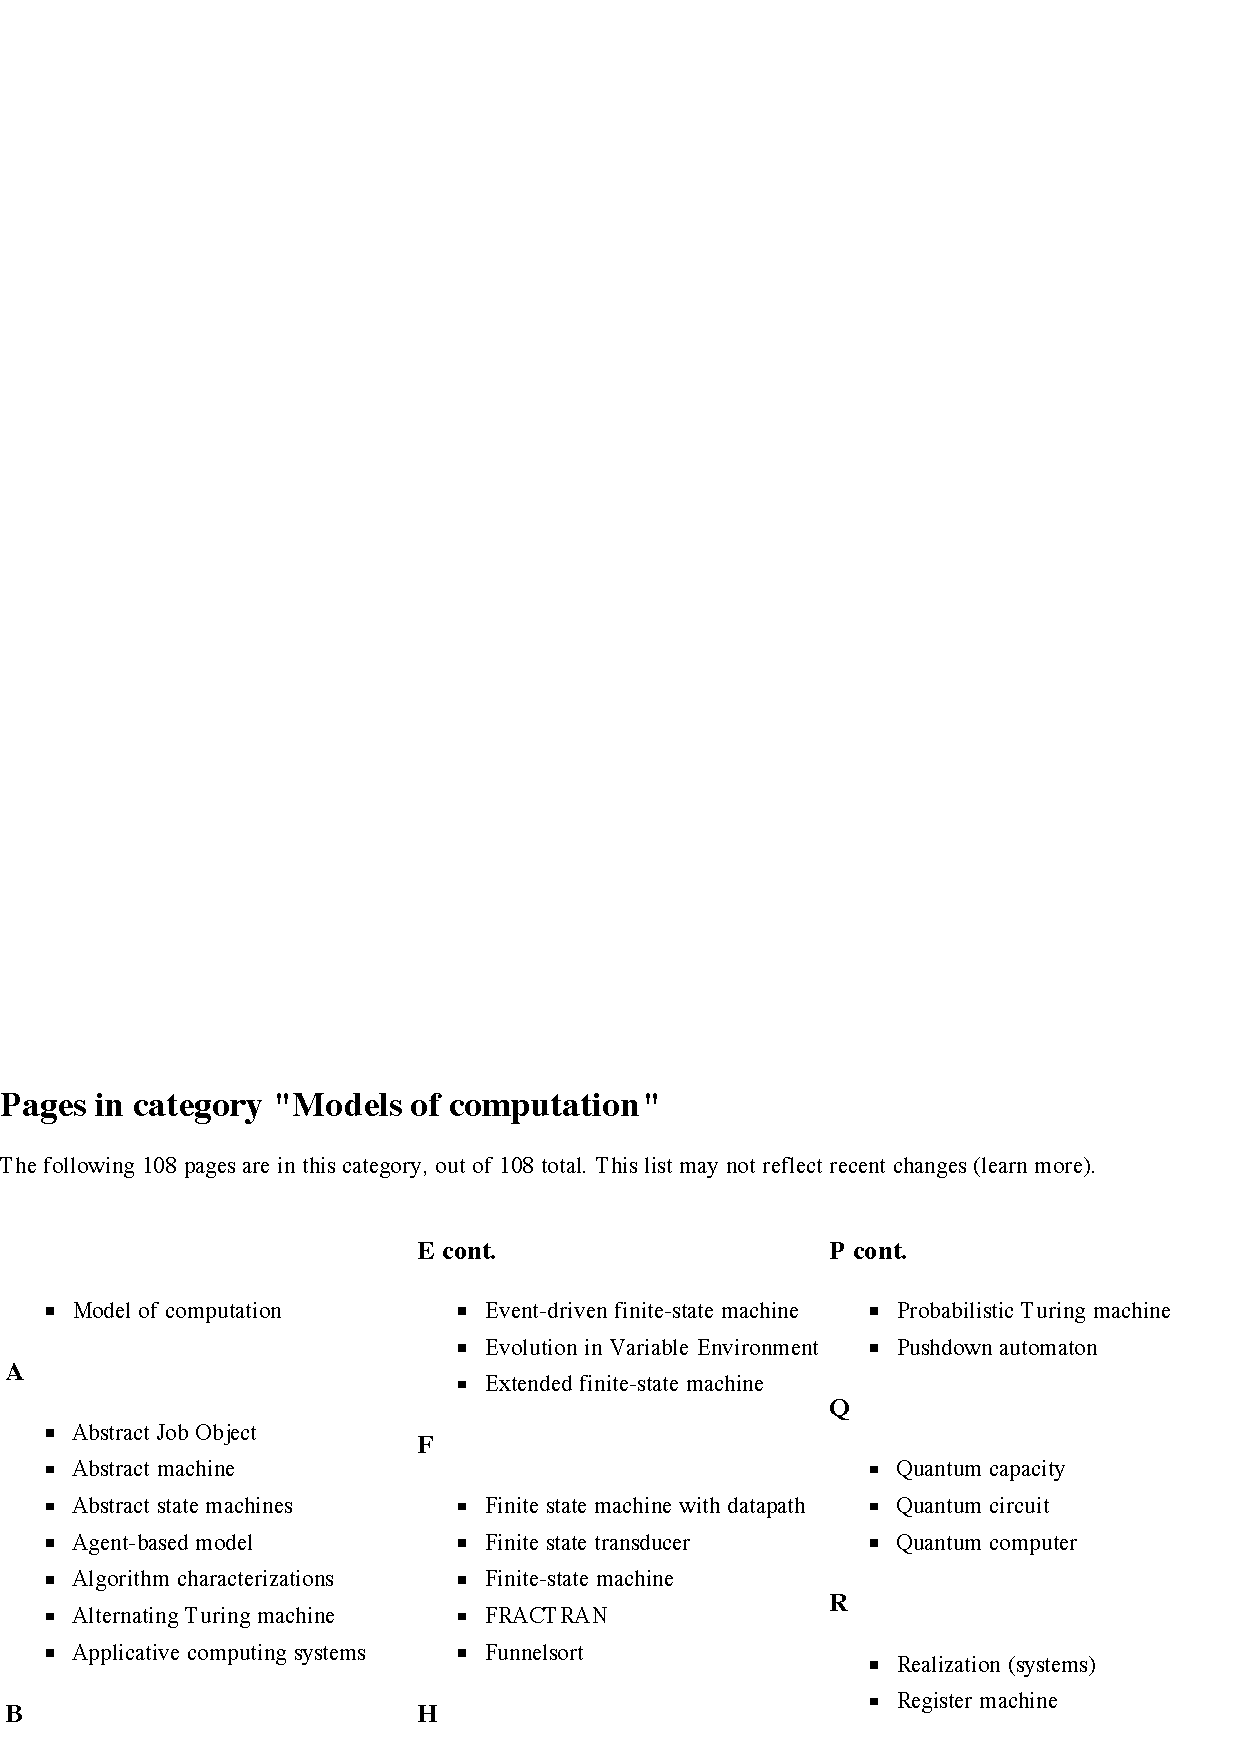
\includegraphics[width=\textwidth]{models.pdf}

\end{frame}

%-------------------------------------------------------------------------
\begin{frame}{Modelli di calcolo}
	
\vspace{-9pt}
\begin{myboxtitle}[Macchina di Turing]
Una macchina ideale che manipola i dati contenuti su un nastro di lunghezza
infinita, secondo un insieme prefissato di regole.
\begin{columns}[T]
\begin{column}{0.28\textwidth}
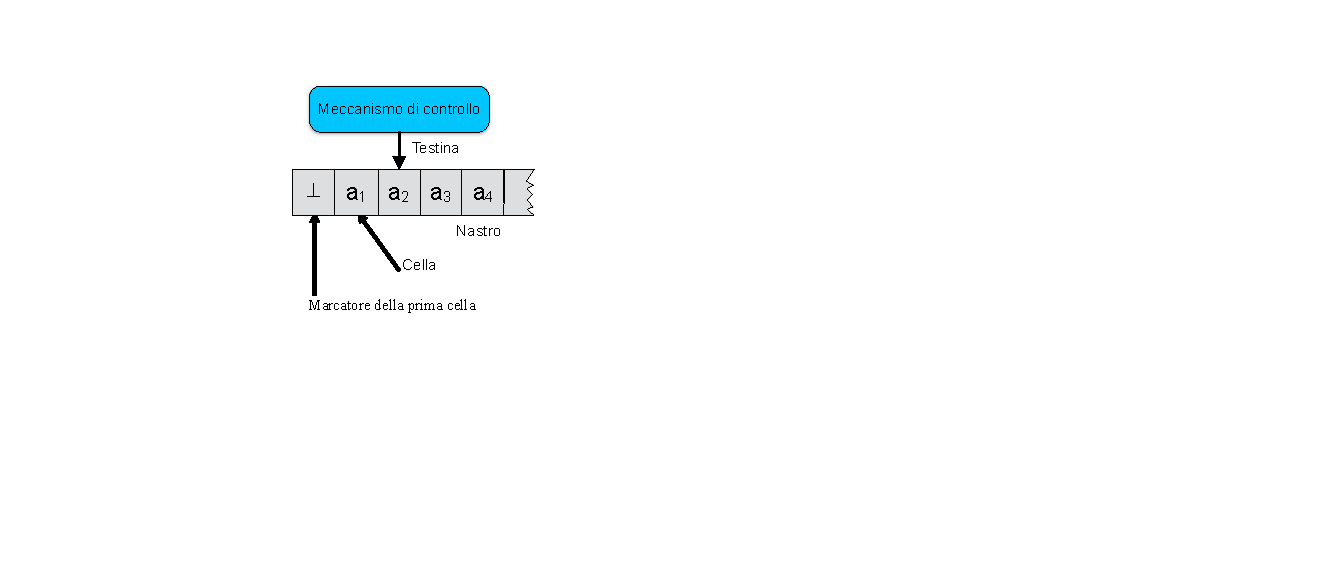
\includegraphics[width=\textwidth]{turing.pdf}
\end{column}
\begin{column}{0.58\textwidth}
~\\
Ad ogni passo, la Macchina di Turing:
\BI
\item legge il simbolo sotto la testina
\item modifica il proprio stato interno
\item scrive un nuovo simbolo nella cella
\item muove la testina a destra o a sinistra
\EI
\end{column}
\end{columns}
\end{myboxtitle}

\smallskip	
\BI
\item Fondamentale nello studio della calcolabilità
\item Livello troppo basso per i nostri scopi
\EI
\end{frame}

%-------------------------------------------------------------------------
\begin{frame}{Modelli di calcolo}
    
\vspace{-9pt}
\begin{myboxtitle}[Random Access Machine (RAM)]
\BI
\item \alert{Memoria}:
\BI
\item Quantità infinita di celle di dimensione finita
\item Accesso in tempo costante (indipendente dalla posizione)
\EI
\item \alert{Processore (singolo)}
\BI
\item Set di istruzioni elementari simile a quelli reali: 
\BI
\item  somme, sottrazioni, moltiplicazioni, operazioni logiche, etc. 
\item istruzioni di controllo (salti, salti condizionati)
\EI
\EI
\item \alert{Costo delle istruzioni elementari}
\BI
\item Uniforme, ininfluente ai fini della valutazione (come vedremo)
\EI
\EI
\end{myboxtitle}
\end{frame}

\subsection{Esempi di analisi}

%-------------------------------------------------------------------------
\begin{frame}{Tempo di calcolo \textsf{min}()}
	
\BI
\item Ogni istruzione richiede un tempo costante per essere eseguita
\item La costante è potenzialmente diversa da istruzione a istruzione
\item Ogni istruzione viene eseguita un certo \# di volte, dipendente da $n$
\EI	
	
	
\begin{Procedure}
~\Rem*[r]{\makebox[15mm][c]{Costo}\makebox[15mm][c]{\# Volte}}
\caption[A]{\Item \MIN($\Item[\,]\ A,\ \INTEGER\ n$)}
\Item $\Min = A[1]$\Rem*[r]{\makebox[15mm][c]{$c_1$}\makebox[15mm][c]{$1$}}
\For(\Rem*[f]{\makebox[15mm][c]{$c_2$}\makebox[15mm][c]{$n$}}){$i = 2$ \TO $n$}
{
   \If(\Rem*[f]{\makebox[15mm][c]{$c_3$}\makebox[15mm][c]{$n-1$}}){$A[i] < \Min$}{ 
      $\Min = A[i]$\Rem*[r]{\makebox[15mm][c]{$c_4$}\makebox[15mm][c]{$n-1$}}
   }
}
\Return $\Min$\Rem*[r]{\makebox[15mm][c]{$c_5$}\makebox[15mm][c]{$1$}}
\end{Procedure}

\vspace{-12pt}
\begin{align*}
T(n) 	&= c_1+c_2n+c_3(n-1)+c_4(n-1)+c_5\\
		&= (c_2+c_3+c_4)n+(c_1+c_5-c_3-c_4) = \alert{an+b}
\end{align*}
\end{frame}

%-------------------------------------------------------------------------
\begin{frame}[shrink=5]{Tempo di calcolo \textsf{binarySearch}()}

\vspace{-9pt}
\begin{columns}
\begin{column}{0.55\textwidth}
Il vettore viene suddiviso in due parti: 
\end{column}
\begin{column}{0.45\textwidth}
Parte SX:  \alert{$\lfloor (n-1)/2 \rfloor$}\\
Parte DX: \alert{$\lfloor n/2 \rfloor$}
\end{column}
\end{columns}

{\footnotesize
\begin{Procedure}
\caption[A]{\INTEGER \binarysearch($\Item[\,]\ A$, $\Item\ v$, \INTEGER $i$, \INTEGER $j$)}
\Rem*[r]{\makebox[25mm][c]{Costo}\makebox[15mm][c]{\# ($i>j$)}\makebox[15mm][c]{\# ($i \leq j$)}}
\uIf(\Rem*[f]{\makebox[25mm][c]{$c_1$}\makebox[15mm][c]{$1$}\makebox[15mm][c]{$1$}}){$i>j$}{
  \Return $0$\Rem*[r]{\makebox[25mm][c]{$c_2$}\makebox[15mm][c]{$1$}\makebox[15mm][c]{$0$}}
}
\Else
{
  \INTEGER $m = \lfloor (i+j)/2 \rfloor$\Rem*[r]{\makebox[25mm][c]{$c_3$}\makebox[15mm][c]{$0$}\makebox[15mm][c]{$1$}}
  \uIf(\Rem*[f]{\makebox[25mm][c]{$c_4$}\makebox[15mm][c]{$0$}\makebox[15mm][c]{$1$}}){$A[m] = v$}{ 
    \Return $m$\Rem*[r]{\makebox[25mm][c]{$c_5$}\makebox[15mm][c]{$0$}\makebox[15mm][c]{$0$}}
  }
  \uElseIf(\Rem*[f]{\makebox[25mm][c]{$c_6$}\makebox[15mm][c]{$0$}\makebox[15mm][c]{$1$}}){$A[m] < v$}{
    \Return $\binarysearch(A, v, m+1, j)$\Rem*[r]{\makebox[25mm][c]{$c_7 + T(\lfloor n/2 \rfloor)$}\makebox[15mm][c]{$0$}\makebox[15mm][c]{$0/1$}}
  }
  \Else {
    \Return $\binarysearch(A, v, i, m-1)$\Rem*[r]{\makebox[25mm][c]{$c_7 + T(\lfloor (n-1)/2 \rfloor)$}\makebox[15mm][c]{$0$}\makebox[15mm][c]{$1/0$}} 
  }
}

\end{Procedure}
}	
\end{frame}

%-------------------------------------------------------------------------
\begin{frame}{Tempo di calcolo \textsf{binarySearch}()}
\BI
\item \alert{Assunzioni} (Caso pessimo):
\BI
\item Per semplicità, assumiamo $n$ potenza di $2$: $n =2^k$
\item L'elemento cercato non è presente 
\item Ad ogni passo, scegliamo sempre la parte DX di dimensione $n/2$ 
\EI
\item \alert{Due casi}:
\begin{columns}[T]
\begin{column}{0.1\textwidth}\end{column}
\begin{column}{0.3\textwidth}
$i>j \quad(n=0)$\\	
~\\
$i\leq j \quad (n>0)$
\end{column}
\begin{column}{0.6\textwidth}
$T(n) = c_1 + c_2 = c$\\
~\\
\makebox[1.2cm][r]{$T(n) =$} $T(n/2) + c_1+c_3+c_4+c_6+c_7$\\
\makebox[1.2cm][r]{$=$} $T(n/2) + d$
\end{column}
\end{columns}
\item \alert{Relazione di ricorrenza}:
\[
T(n) = \begin{cases}
c  & \textrm{se $n=0$}\\
T(n/2) + d & \textrm{se $n\ge1$}
\end{cases}
\]
\EI
\end{frame}

%-------------------------------------------------------------------------
\begin{frame}{Tempo di calcolo \textsf{binarySearch}()}
Soluzione della relazione di ricorrenza tramite espansione
\begin{columns}[c]
\begin{column}{0.5\textwidth}
\begin{align*}
T(n) 	&= T(n/2) + d\\
		&= T(n/4) + 2d\\
		&= T(n/8) + 3d\\
		& \ldots\\
		&= T(1) + kd\\
		&= T(0) + (k+1)d\\
		&= kd+(c+d) \\
		&= d \log n + e.
\end{align*}
\end{column}
\begin{column}{0.3\textwidth}
\begin{beamerboxesrounded}[shadow=true]{}
\begin{center}
$n = 2^k \Rightarrow k = \log n$
\end{center}
\end{beamerboxesrounded}
\end{column}
\begin{column}{0.2\textwidth}
\end{column}
\end{columns}

\end{frame}

\subsection{Ordini di complessità}

%-------------------------------------------------------------------------
\begin{frame}{Ordini di complessità}
	
Per ora, abbiamo analizzato precisamente due algoritmi e abbiamo ottenuto due \emph{funzioni di complessità}:
\BI
\item \onslide<1->\makebox[6cm][l]{Ricerca: $T(n) = d \log n + e$}  \onslide<2->\makebox[2.5cm][l]{\alert{logaritmica}} \alert{$O(\log n)$}
\item \onslide<1->\makebox[6cm][l]{Minimo: $T(n) = an + b$}  \onslide<2-> \makebox[2.5cm][l]{\alert{lineare}} \alert{$O(n)$}
\EI

\onslide<3->
\medskip
Una terza funzione deriva dall'\emph{algoritmo naïf} per il minimo:
\BI
\item \makebox[6cm][l]{Minimo: $T(n) = f n^2 + gn +h$} \makebox[2.5cm][l]{\alert{quadratica}} \alert{$O(n^2)$}
\EI

% \onslide<4->
% \bigskip
% \begin{myboxtitle}[Notazione \alert{$O(f(n))$} -- Limite superiore]
% Un algoritmo ha complessità \alert{$O(f(n))$} se il suo tempo di esecuzione è \alert{limitato superiormente}
% da una funzione di complessità $c \cdot f(n)$, dove $c$ è un'opportuna costante.
% \end{myboxtitle}
	
\end{frame}

%-------------------------------------------------------------------------
\begin{frame}{Classi di complessità}


\begin{center}
\begin{tabular}{|c|c|c|c|c|c|}
\hline
$f(n)$ & $n=10^1$ & $n=10^2$ & $n=10^3$ & $n=10^4$ & \textbf{Tipo} \\
\hline
$\log n$ & 3 & 6 & 9 & 13 & logaritmico \\
\hline
$\sqrt{n}$ & 3 & 10 & 31 & 100 & sublineare \\
\hline
$n$ & 10 & 100 & 1000 & 10000 & lineare \\
\hline
$n \log n$ & 30 & 664 & 9965 & 132877 & loglineare \\
\hline
$n^2$ & $10^2$ & $10^4$ & $10^6$ & $10^8$& quadratico \\
\hline
$n^3$ & $10^3$ & $10^6$ & $10^9$ & $10^{12}$ & cubico \\
\hline
$2^n$ & 1024 & $10^{30}$ & $10^{300}$ & $10^{3000}$ & esponenziale \\
\hline
\end{tabular}
\end{center}

\bigskip
Come sbagliare completamente l'algoritmo di controllo degli update in
Windows XP e renderlo esponenziale:
\url{http://m.slashdot.org/story/195683}


\end{frame}


\input analisi/funzioni-1.tex

\title[ASD - Analisi di algoritmi]{\textbf{Algoritmi e strutture dati}\\[12pt]Analisi di algoritmi\\Complessità algoritmi vs Complessità problemi}

%-------------------------------------------------------------------------
\FrameTitle{}

\section{Complessità problemi vs algoritmi}


%-------------------------------------------------------------------------
\begin{frame}{Introduzione}

\vspace{-9pt}
\begin{myboxtitle}[Obiettivo: \alert{riflettere su complessità di problemi/algoritmi}]

\BI
\item In alcuni casi, si può migliorare quanto si ritiene "normale"
\item In altri casi, è impossibile fare di meglio
\item Qual è il rapporto fra un problema computazionale e l'algoritmo?
\EI
\end{myboxtitle}

\begin{myboxtitle}[Back to basics!]
\BI
\item Somme 
\item Moltiplicazioni
\EI
\end{myboxtitle}


\end{frame}

\subsection{Moltiplicare numeri complessi}


%-------------------------------------------------------------------------
\begin{frame}{Moltiplicare numeri complessi}

\vspace{-9pt}
\begin{myboxtitle}[Moltiplicazione numeri complessi]
\BI
\item $(a + bi)(c + di) = [ac-bd] + [ad + bc] i$
\item Input: $a$, $b$, $c$, $d$
\item Output: $ac-bd$, $ad+bc$
\EI
\end{myboxtitle}

\begin{myboxtitle}[Domande]
Considerate un modello di calcolo dove la moltiplicazione costa $1$, le addizioni/sottrazioni costano $0.01$,
\BI
\item Quanto costa l'algoritmo dettato dalla definizione?
\item Potete fare meglio di così? 
\item Qual è il ruolo del modello di calcolo?
\EI
\end{myboxtitle}	

\end{frame}

%-------------------------------------------------------------------------
\begin{frame}{Moltiplicare numeri complessi}

\vspace{-9pt}
\begin{myboxtitle}[Questioni aperte]
\BI
\item Si può fare ancora meglio? 
\item Oppure, è possibile dimostrare che non si può fare meglio di così?
\EI
\end{myboxtitle}

\begin{myboxtitle}[Alcune riflessioni]
\BI
\item In questo modello, effettuare 3 moltiplicazioni invece di 4 risparmia il 25\% del costo
\item Esistono contesti in cui effettuare 3 moltiplicazioni invece di 4 può produrre un risparmio maggiore
\EI
\end{myboxtitle}

\end{frame}

\subsection{Sommare numeri binari}

%-------------------------------------------------------------------------
\begin{frame}{Sommare numeri binari}

\vspace{-9pt}
\begin{myboxtitle}[Algoritmo elementare della somma -- \textsf{sum}()]
\BI
\item richiede di esaminare tutti gli $n$ bit
\item costo totale $cn = O(n)$ \\
  ($c \equiv$ costo per sommare tre bit e generare riporto)
\EI
\end{myboxtitle}

\begin{myboxtitle}[Domanda]
Esiste un metodo più efficiente?
\end{myboxtitle}

\begin{center}
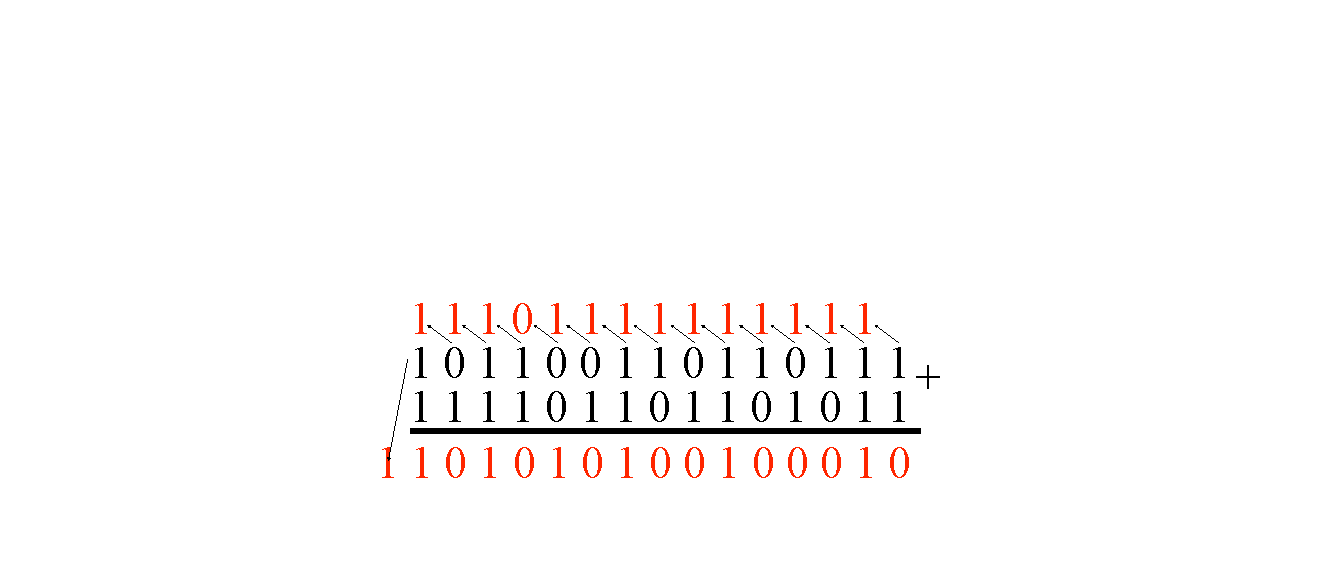
\includegraphics[width=10cm]{sum.pdf}
\end{center}

\end{frame}

%-------------------------------------------------------------------------
\begin{frame}{Limite superiore alla complessità di un problema}

\vspace{-9pt}
\begin{myboxtitle}[Notazione $O(f(n))$ -- Limite superiore]
Un problema ha complessità $O(f(n))$ se esiste almeno un algoritmo
che ha complessità $O(f(n))$
\end{myboxtitle}

\bigskip
\begin{myboxtitle}[Limite superiore della somma di numeri binari]
Il problema della somma di numeri binari ha complessità $O(n)$.
\end{myboxtitle}



\end{frame}


%-------------------------------------------------------------------------
\begin{frame}{Limite inferiore alla complessità di un problema}

\vspace{-9pt}
\begin{myboxtitle}[Notazione $\Omega(f(n))$ -- Limite inferiore]
Un problema ha complessità $\Omega(f(n))$ se tutti i possibili algoritmi che lo risolvono hanno complessità $\Omega(f(n))$.
\end{myboxtitle}

\bigskip
\begin{myboxtitle}[Limite inferiore della somma di numeri binari]
Il problema della somma di numeri binari ha complessità $\Omega(n)$.
\end{myboxtitle}

\begin{myboxtitle}[Domanda]
Riuscite a dimostrarlo?
\end{myboxtitle}

\end{frame}

\subsection{Moltiplicare numeri binari}

%-------------------------------------------------------------------------
\begin{frame}{Moltiplicare numeri binari}

\vspace{-9pt}
\begin{myboxtitle}[Algoritmo elementare del prodotto -- \textsf{prod}()]
\BI
\item moltiplicazione di ogni bit con ogni altro bit
\item costo totale $cn^2 = O(n^2)$
\EI
\end{myboxtitle}

\begin{center}
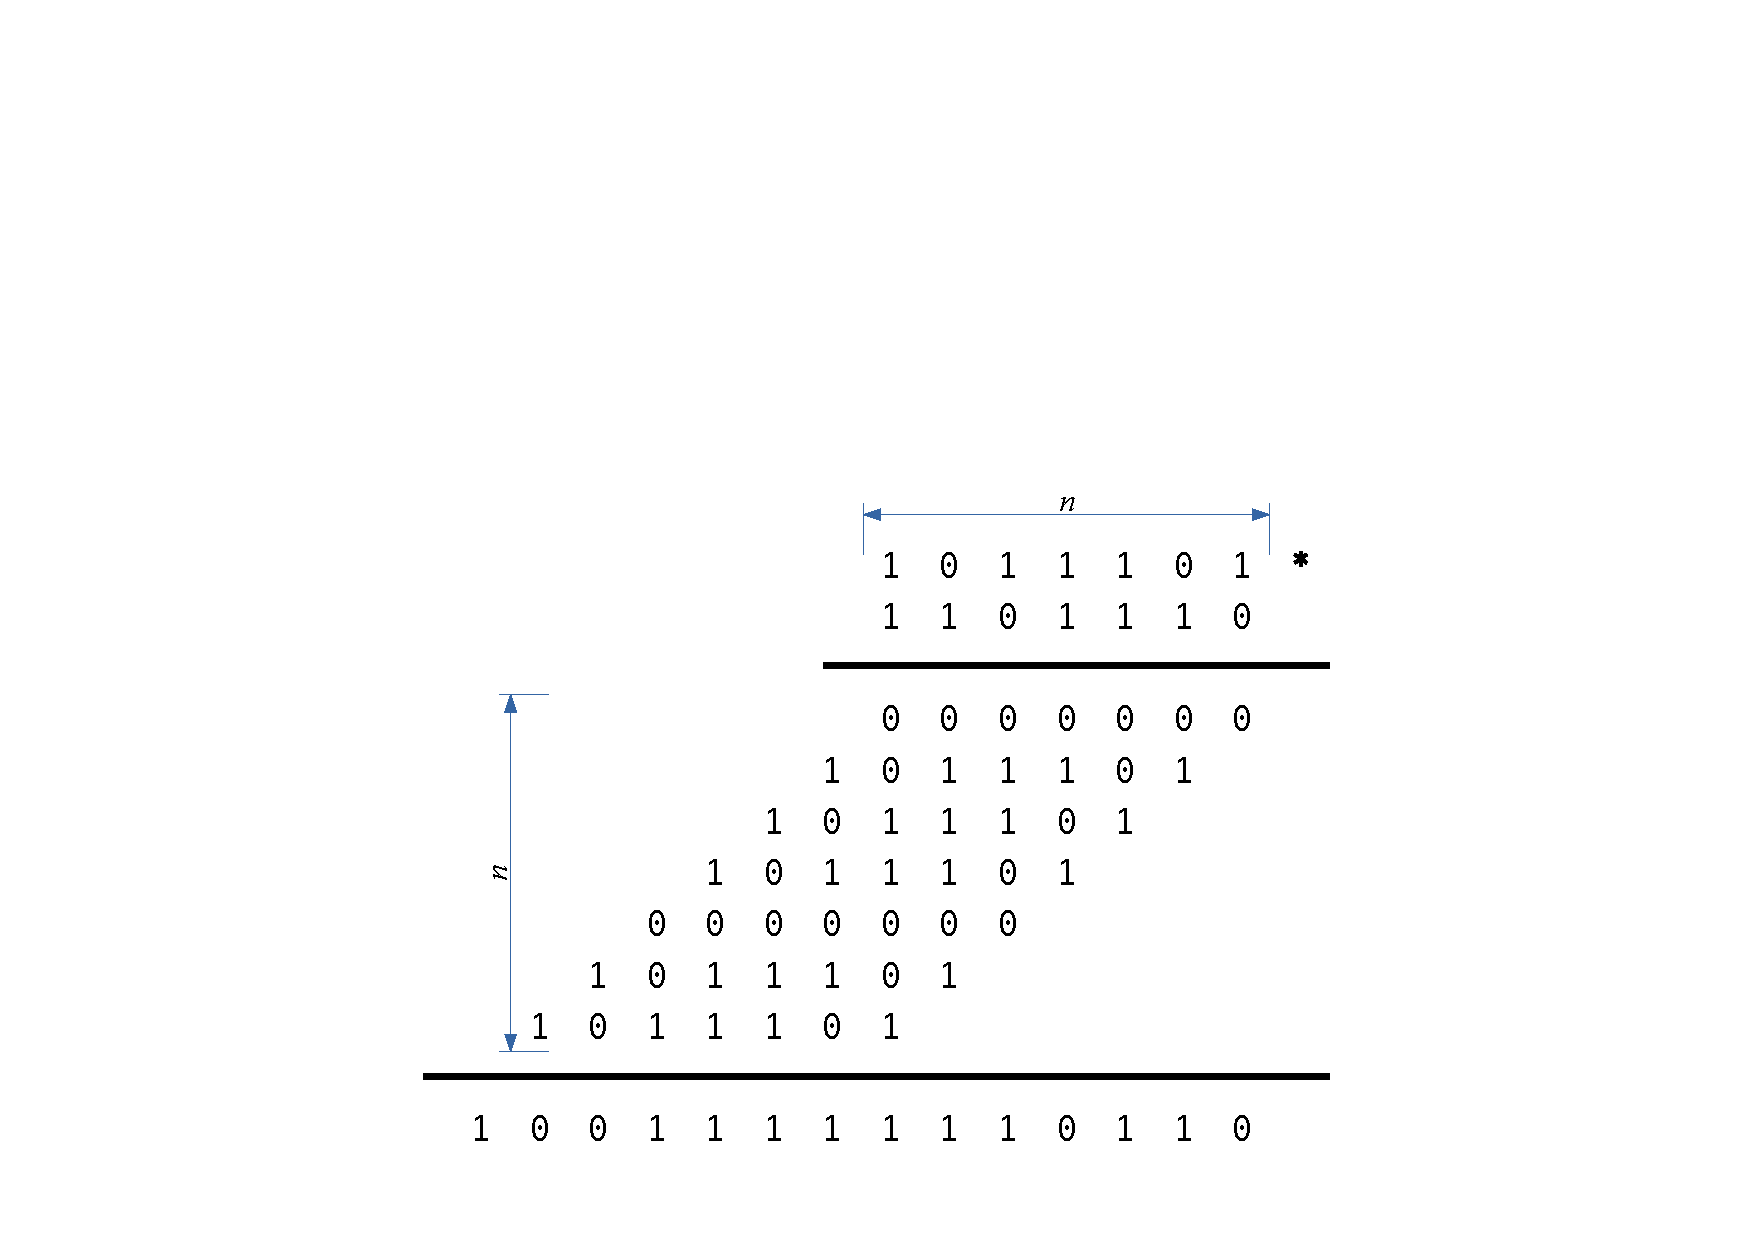
\includegraphics[width=7.5cm]{multiplication.pdf}
\end{center}

\end{frame}

%-------------------------------------------------------------------------
\begin{frame}{Algoritmi aritmetici}

\vspace{-9pt}
\begin{myboxtitle}[Confronto della complessità computazionale]
\BI
\item \makebox[1.6cm][l]{Somma}: $T_{sum}(n) = O(n)$
\item \makebox[1.6cm][l]{Prodotto}: $T_{prod}(n) = O(n^2)$
\EI
\end{myboxtitle}

\bigskip
Si potrebbe concludere che...
\BI
\item Il problema della moltiplicazione è inerentemente più costoso del problema dell'addizione
\item Conferma la nostra esperienza
\EI

\end{frame}

%-------------------------------------------------------------------------
\begin{frame}{Algoritmi aritmetici}

\vspace{-9pt}
\begin{myboxtitle}[Confronto fra problemi]
Per provare che il problema del prodotto è più costoso del problema della somma, dobbiamo provare che \alert{non esiste} una soluzione in tempo sub-quadratico per il prodotto
\end{myboxtitle}

\BB{
\BI
\item Abbiamo confrontato gli algoritmi, non i problemi!
\item Sappiamo solo che l'algoritmo di somma delle elementari è più efficiente dell'algoritmo del prodotto delle elementari
\EI
}

\begin{myboxtitle}[Un po' di storia]
\BI
\item Nel 1960, Kolmogorov enunciò in una conferenza che la moltiplicazione ha limite inferiore $\Omega(n^2)$
\item Una settimana dopo, un suo studente provò il contrario!
\EI
\end{myboxtitle}


\end{frame}

%-------------------------------------------------------------------------
\begin{frame}{Moltiplicare numeri binari}

\vspace{-9pt}
\begin{myboxtitle}[Divide-et-impera]
\BI
\item \alert{Divide}: dividi il problema in sottoproblemi di dimensioni inferiori
\item \alert{Impera}: risolvi i sottoproblemi in maniera ricorsiva
\item \alert{Combina}: unisci le soluzioni dei sottoproblemi in modo da ottenere la risposta del problema principale
\EI
\end{myboxtitle}

\begin{myboxtitle}[Moltiplicazione divide-et-impera]
\begin{columns}[c]
\begin{column}{0.52\textwidth}
\begin{align*}
X &= a \cdot 2^{n/2} + b  \\
Y &= c \cdot 2^{n/2} + d\\
XY &= ac \cdot 2^n + (ad+bc) \cdot 2^{n/2} + bd
\end{align*}
\end{column}
\begin{column}{0.46\textwidth}
\begin{center}
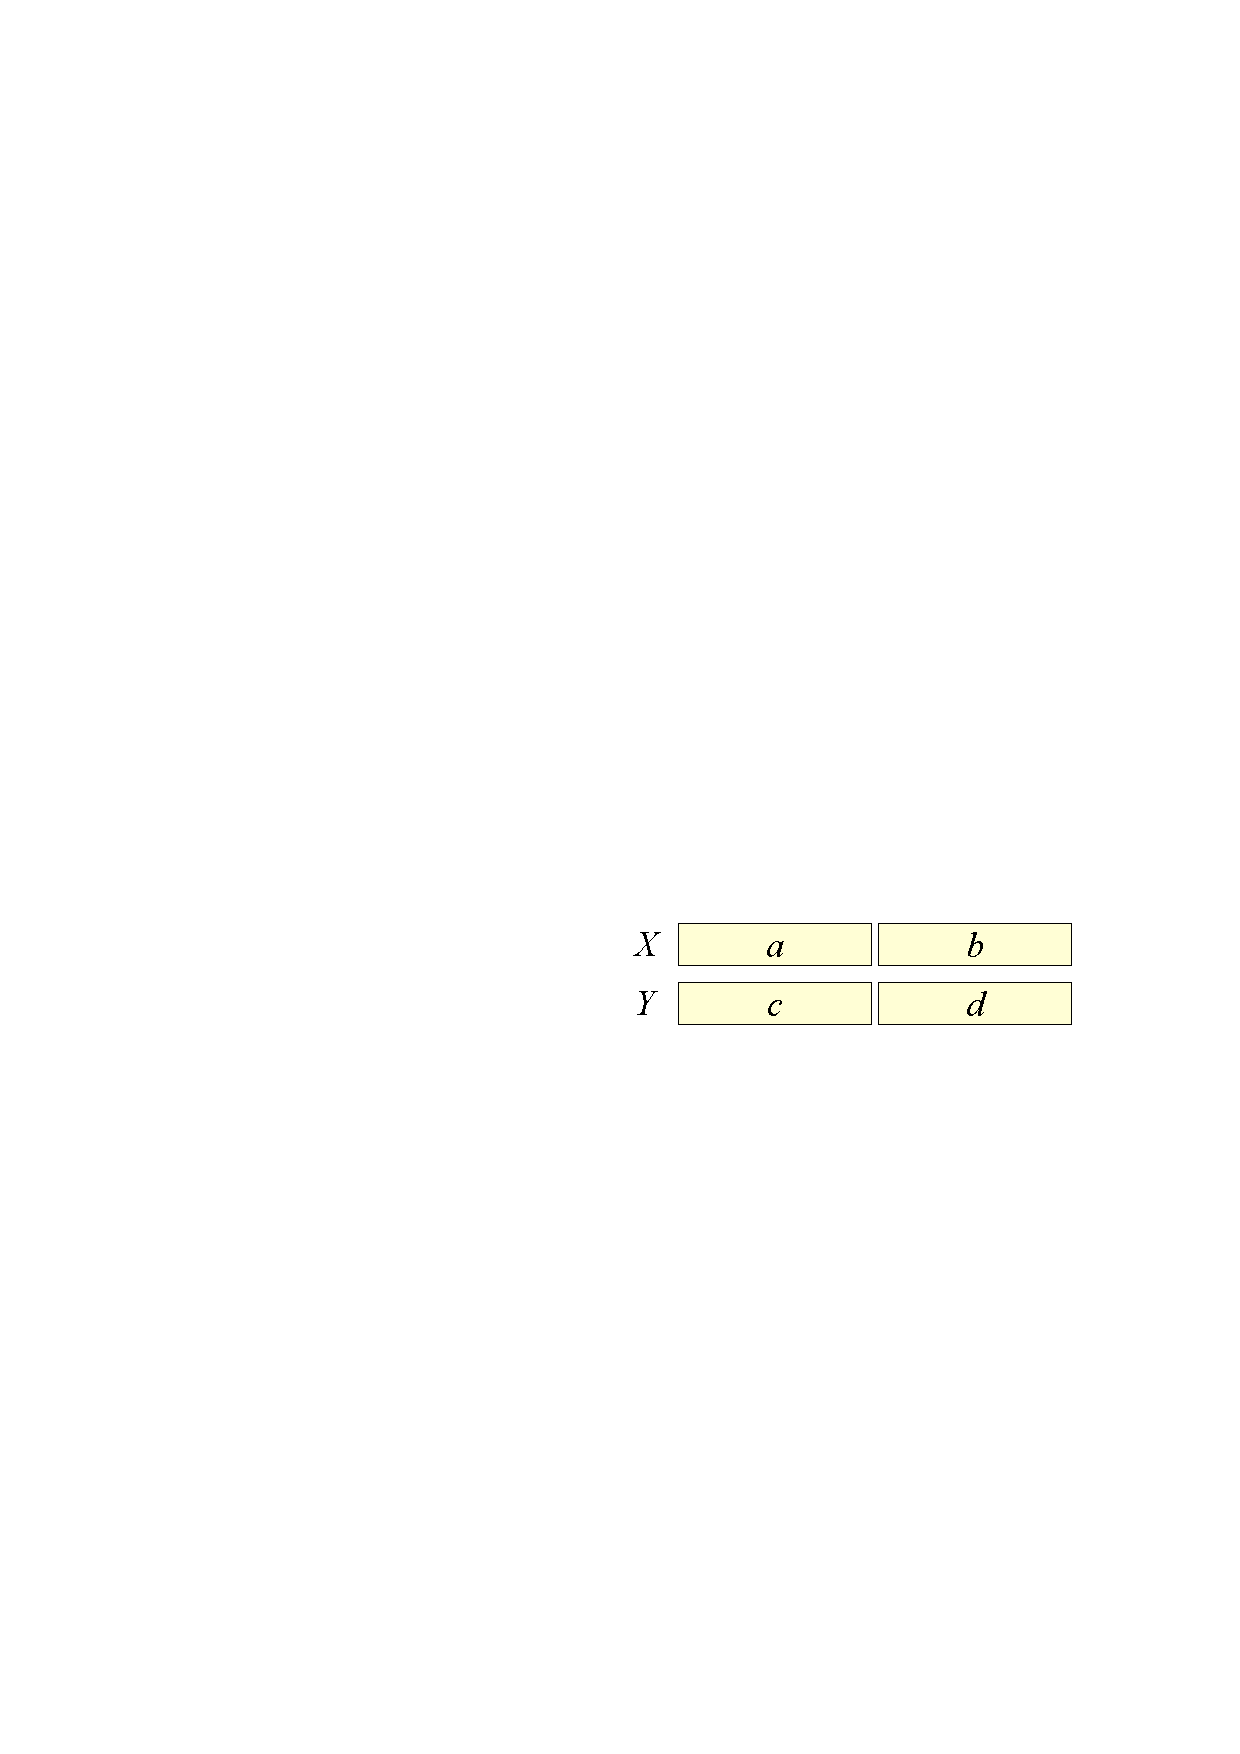
\includegraphics[width=0.95\textwidth]{mul-di.pdf}
\end{center}
\end{column}
\end{columns}
\end{myboxtitle}


\end{frame}

%-------------------------------------------------------------------------
\begin{frame}{Moltiplicare numeri binari tramite Divide-et-impera}
    
\vspace{-9pt}
\begin{Procedure}
\caption[A]{$\BOOLEAN[\,]\ \textsf{pdi}(\BOOLEAN[\,]\ X,\ \BOOLEAN[\,]\ Y,\ \INTEGER\ n)$}
\eIf{$n \Eq 1$}{
  \Return $X[1] \cdot Y[1]$\;
}
{
  spezza $X$ in $a;b$ e $Y$ in $c;d$\;
  \Return $\textsf{pdi}(a,c, n/2)\cdot 2^n + (\textsf{pdi}(a,d, n/2)+$\; 
  \hspace{1.2cm} $\textsf{pdi}(b,c, n/2)) \cdot 2^{n/2} + \textsf{pdi}(b,d, n/2)$\;
}
\end{Procedure}
\[
T(n) = \left\{ 
  \begin{array}{ll}
     c_1 & n = 1\\
     4 T(n/2) + c_2 \cdot n & n > 1 
  \end{array} 
\right.
\]


\begin{mybox}
\alert{Nota}:
 Moltiplicare per $2^t$ $\equiv$ shift di $t$ posizioni, in tempo lineare
\end{mybox}

	
\end{frame}

%-------------------------------------------------------------------------
\begin{frame}{Analisi della ricorsione}

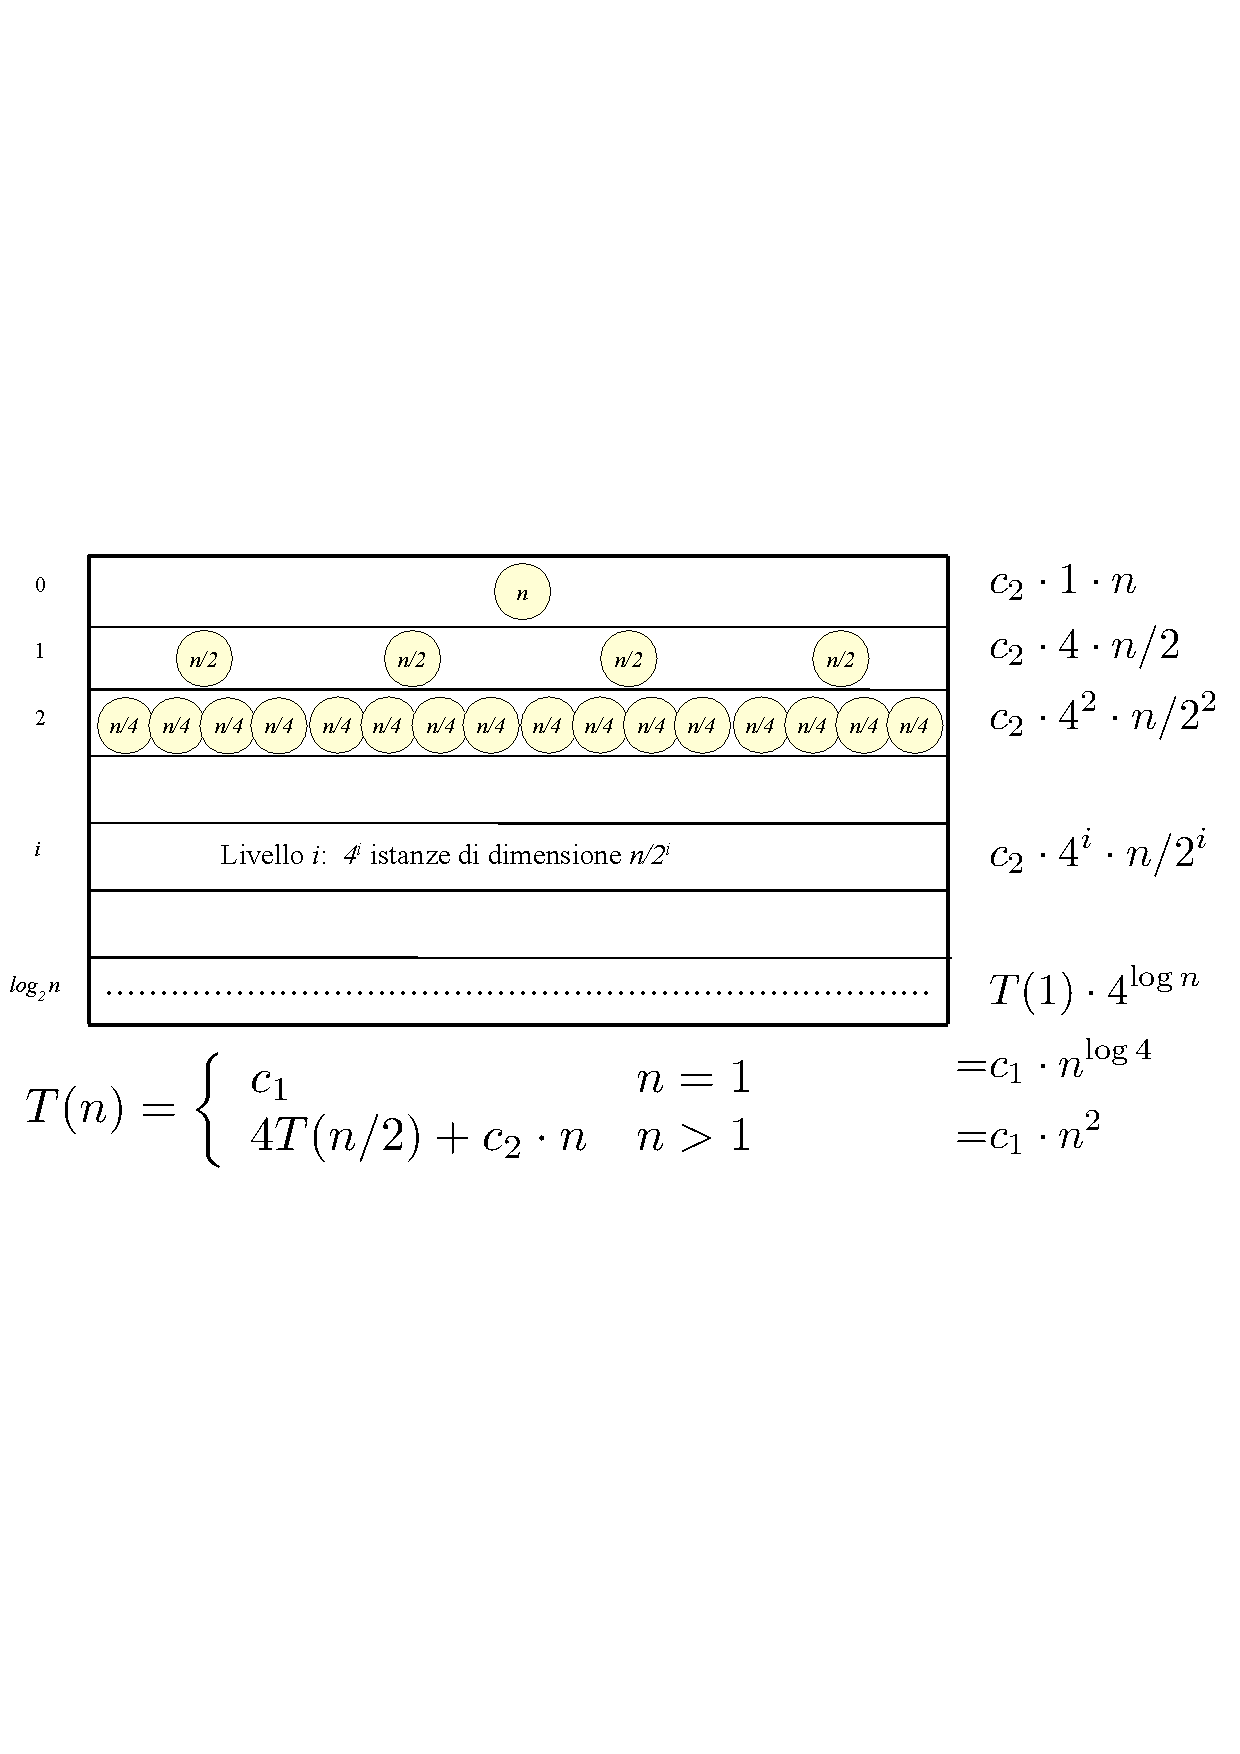
\includegraphics[width=\textwidth]{ricorsione.pdf}

\end{frame}

%-------------------------------------------------------------------------
\begin{frame}{Moltiplicare numeri binari}

\vspace{-9pt}
\begin{myboxtitle}[Confronto della complessità computazionale]
\BI
\item \makebox[1.6cm][l]{Prodotto}: $T_{prod}(n) = O(n^2)$
\item \makebox[1.6cm][l]{Prodotto}: $T_{pdi}(n) = O(n^2)$
\EI
\end{myboxtitle}

\smallskip
\begin{myboxtitle}[Domanda: Tutto questo lavoro per nulla?]
Non solo la complessità è uguale, ma le costanti moltiplicative 
sono più alte.	
\end{myboxtitle}

\smallskip
\begin{myboxtitle}[Domanda: E' possibile fare meglio di così?]
Notate che la versione ricorsiva chiama se stessa $4$ volte.
\end{myboxtitle} 

\end{frame}

%-------------------------------------------------------------------------
\begin{frame}[shrink=5]{Moltiplicazione di Karatsuba (1962)}

\vspace{-12pt}
\TwoColsCustom{0.6}{0.35}{
\begin{align*}
A_1 &= a \alert{\times} c\\
A_3 &= b \alert{\times} d\\
m &= (a\alert{+}b) \alert{\times} (c\alert{+}d)=ac+ad+bc+bd\\
A_2 &= m\alert{-}A_1\alert{-}A_3=ad+bc
\end{align*}
}{
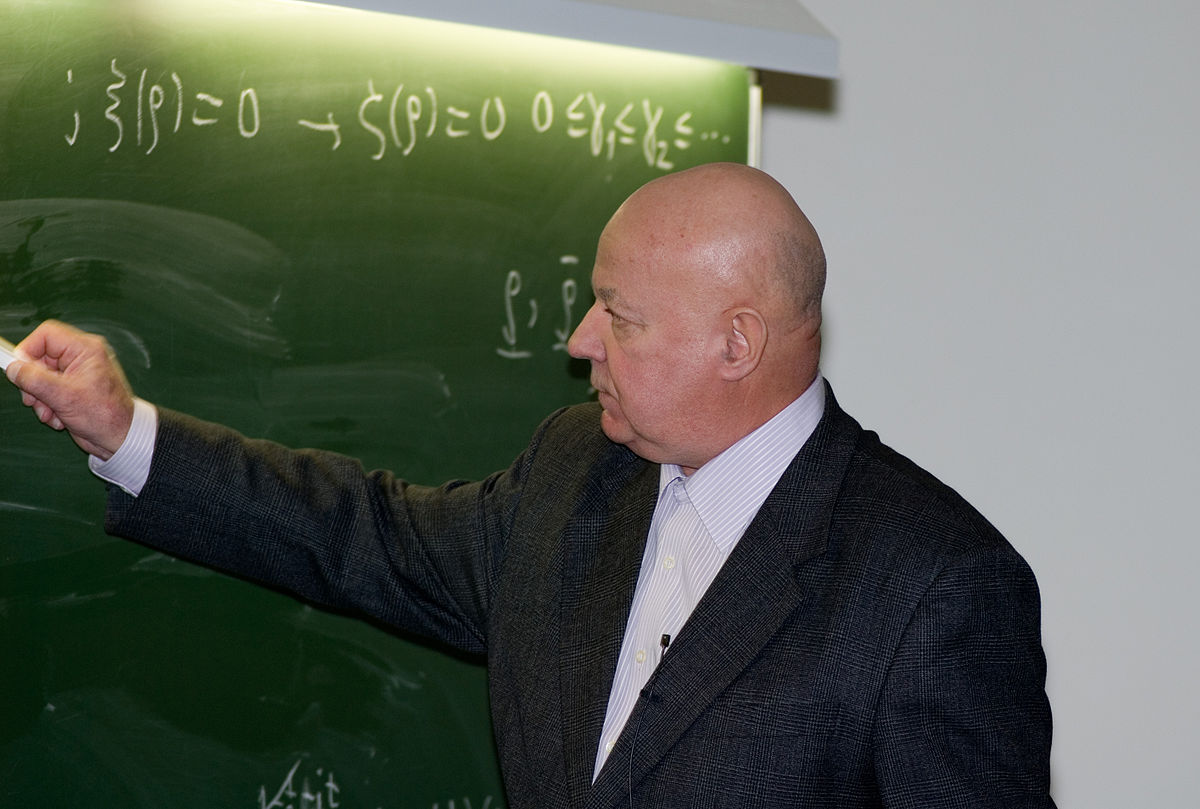
\includegraphics[width=0.8\textwidth]{karatsuba.jpg}
}

\begin{Procedure}
\caption[A]{\BOOLEAN[\,] \textsc{karatsuba}($\BOOLEAN[\,]\ X$, $\BOOLEAN[\,]\ Y$, \INTEGER $n$)}
\eIf{$n \Eq 1$}{
  \Return $X[1] \cdot Y[1]$\;
}
{
  spezza $X$ in $a;b$ e $Y$ in $c;d$\;
  $\BOOLEAN[\,]\ A_1 = \textsc{karatsuba}(a,c, n/2)$\;
  $\BOOLEAN[\,]\ A_3 = \textsc{karatsuba}(b,d, n/2)$\;
  $\BOOLEAN[\,]\ m  = \textsc{karatsuba}(a+b,c+d, n/2)$\;
  $\BOOLEAN[\,]\ A_2 = m-A1-A3$\;
  \Return $A_1\cdot 2^n + A_2 \cdot 2^{n/2} + A_3$\;
}
\end{Procedure}

\end{frame}

%-------------------------------------------------------------------------
\begin{frame}{Analisi della ricorsione}

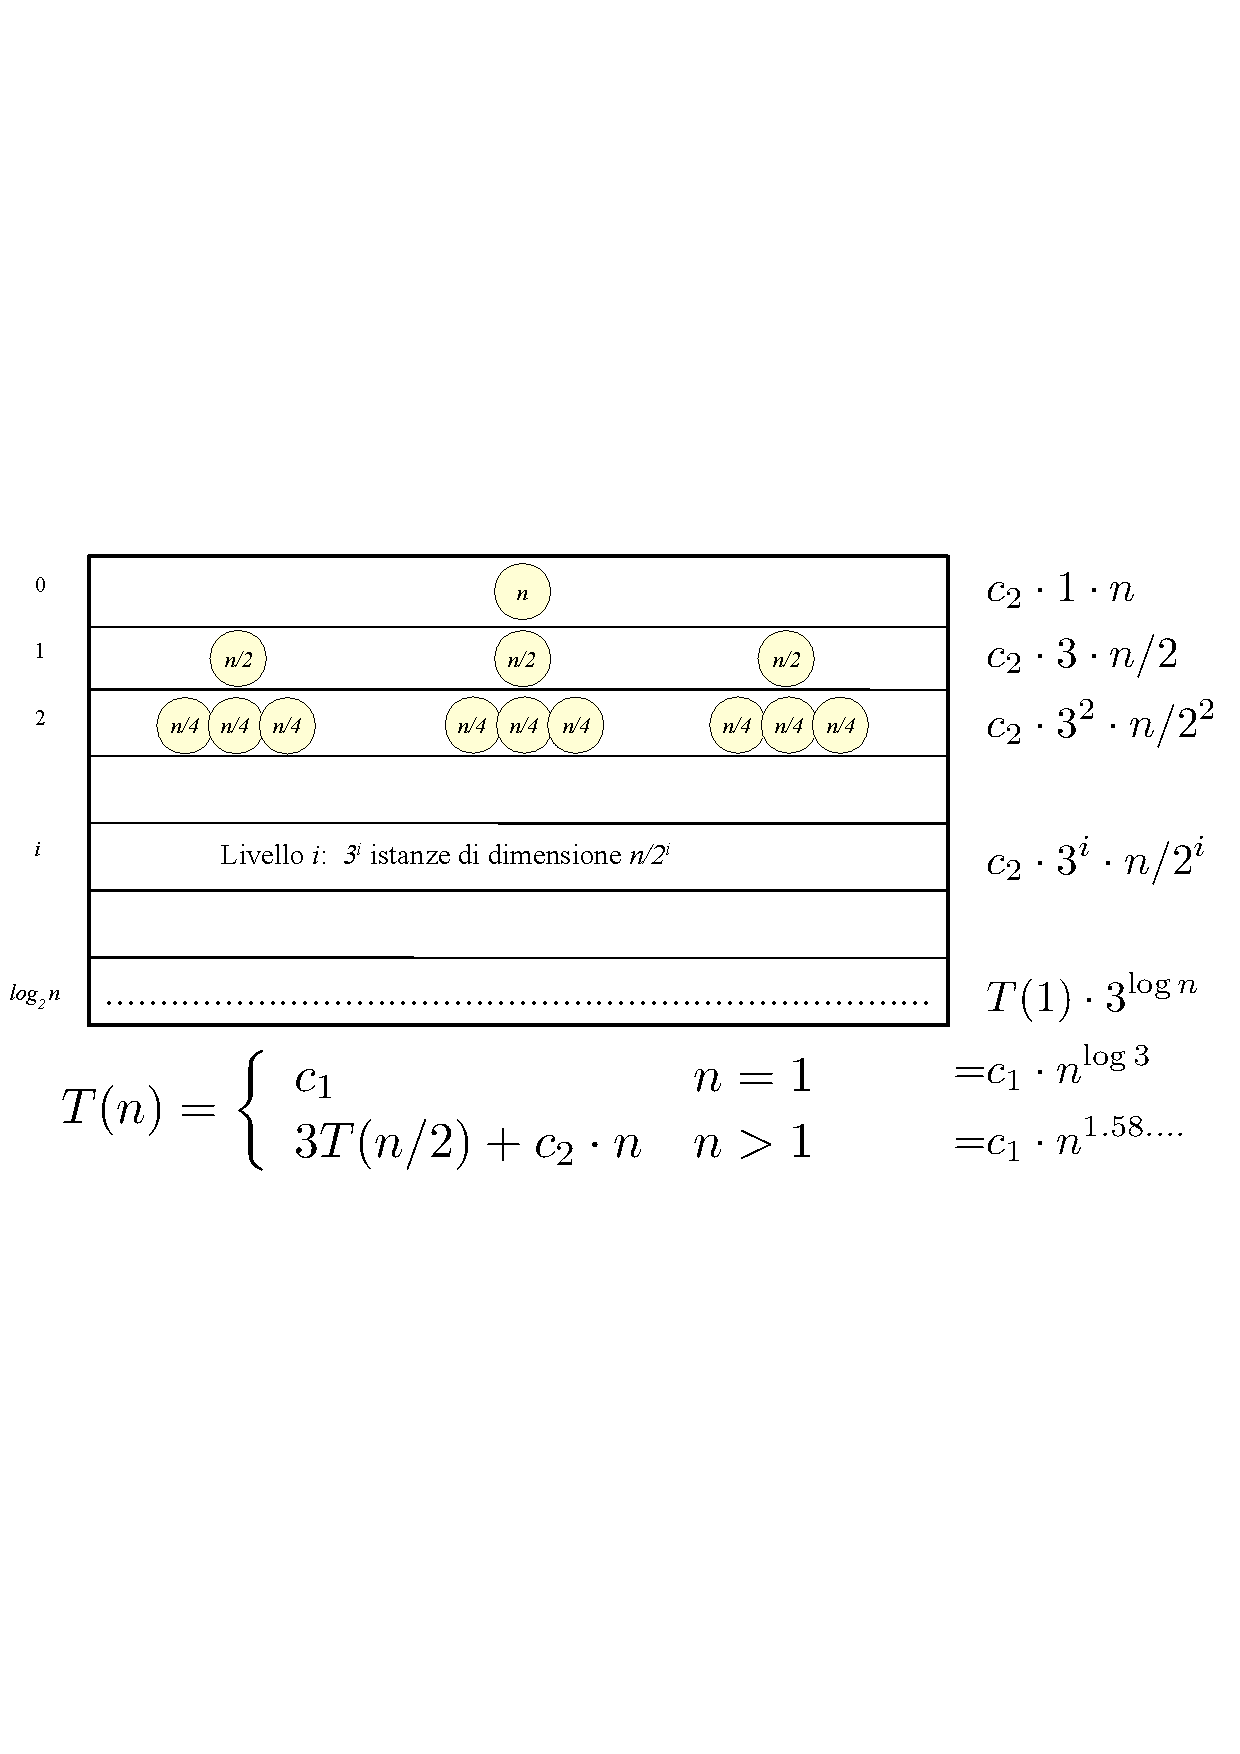
\includegraphics[width=\textwidth]{karatsuba.pdf}

\end{frame}


%-------------------------------------------------------------------------
\begin{frame}{Moltiplicare numeri binari}
    
\vspace{-9pt}
\begin{myboxtitle}[Confronto della complessità computazionale]
\BIL
\item \makebox[1.6cm][l]{Prodotto}: \makebox[4cm][l]{$T_{prod}(n) = O(n^2)$} Es. $T_{prod}(10^6) = 10^{12}$
\item \makebox[1.6cm][l]{Prodotto}: \makebox[4cm][l]{$T_{kara}(n) = O(n^{1.58\ldots})$} Es. $T_{kara}(10^6) = 3 \cdot 10^9$
\EIL
\end{myboxtitle}

\begin{myboxtitle}[Conclusioni]
\BIL
\item L'algoritmo "naif" non è sempre il migliore ...
\item ... può esistere spazio di miglioramento ...
\item ... a meno che non sia possibile dimostrare il contrario!
\EIL
\end{myboxtitle}

\end{frame}

%-------------------------------------------------------------------------
\begin{frame}{Non finisce qui \ldots}

\vspace{-15pt}
\TwoColsCustom{0.60}{0.35}{
\BI
\item \alert{Toom-Cook} (1963)
  \BI
  \item Detto anche Toom3, ha complessità $O(n^{\log 5/\log 3}) \approx  O(n^{1.465})$
  \item Karatsuba $\equiv$ Toom2
  \item Moltiplicazione normale $\equiv$ Toom1
  \EI
\item \alert{Schönhage--Strassen} (1971)
  \BI
  \item Complessità $O(n \cdot \log n \cdot \log \log n)$
  \item Basato su Fast Fourier Transforms
  \EI
\EI
}{
\alert{Crescita funzioni}

\smallskip
\begin{tabular}{|l|l|l|}
\hline
$n$ & $\log^* n$  & $\log \log n$\\\hline
$1$ & 0 & \\\hline
$2$ & 1 & 0\\\hline
$4$ & 2 & 1 \\\hline
$16$ & 3 & 2 \\\hline
$2^{16}$ & 4 & 4  \\\hline
$2^{2^{16}}$ & 5 & 16 \\\hline
\end{tabular}
}
\BI
\item \alert{Fürer} (2007)
  \BI
  \item Complessità $O(n \cdot \log n \cdot K^{O(\log^* n)})$, per qualche $K>1$
  \EI
\item \alert{Harvey--van der Hoeven--Lecerf} (2014)
  \BI
  \item Complessità $O(n \cdot \log n \cdot 8^{O(\log^* n)})$
  \EI
\item \alert{Harvey--van der Hoeven} (2019-2021)
  \BI
  \item Complessità $O(n \cdot \log n)$ (\href{https://hal.archives-ouvertes.fr/hal-02070778/document}{[Articolo]}\href{https://www.youtube.com/watch?v=FKGRc867j10&ab_channel=MathsStatsUNSW}{[Video]})
  \EI
\item Limite inferiore: $\Omega(n \log n)$ (congettura)
\EI

\end{frame}

\begin{frame}{Algoritmi vs problemi}

\vspace{-9pt}
\begin{myboxtitle}[Complessità in tempo di un \alert{algoritmo}]
{\em La quantità di tempo richiesta per input di dimensione $n$}
\BI
\item \alert{$O(f(n))$}: Per tutti gli input, l'algoritmo costa al più $f(n)$ 
\item \alert{$\Omega(f(n))$}: Per tutti gli input, l'algoritmo costa almeno $f(n)$ 
\item \alert{$\Theta(f(n))$}: L'algoritmo richiede $\Theta(f(n))$ per tutti gli input
\EI
\end{myboxtitle}

\begin{myboxtitle}[Complessità in tempo di un \alert{problema computazionale}]
{\em La complessità in tempo relative a tutte le possibili soluzioni}
\BI
\item \alert{$O(f(n))$}: Complessità del miglior algoritmo che risolve il 
problema
\item \alert{$\Omega(f(n))$}: Dimostrare che nessun algoritmo può risolvere il problema in tempo inferiore a $\Omega(f(n))$
\item \alert{$\Theta(f(n))$}: Algoritmo ottimo
\EI
\end{myboxtitle}



\end{frame}



\title[ASD - Analisi di algoritmi]{\textbf{Algoritmi e strutture dati}\\[12pt]Analisi di algoritmi\\Algoritmi di ordinamento}

\FrameTitle

\section{Tipologia dell'input}

%-------------------------------------------------------------------------
\begin{frame}{Introduzione}

\vspace{-9pt}
\begin{myboxtitle}[Obiettivo: \alert{valutare gli algoritmi in base all'input}]
\BI
\item In alcuni casi, gli algoritmi si comportano diversamente a seconda delle caratteristiche dell'input
\item Conoscere in anticipo tali caratteristiche permette di scegliere il miglior algoritmo in quella situazione
\item Il problema dell'ordinamento è una buona palestra dove mostrare questi concetti
\EI
\end{myboxtitle}

\begin{myboxtitle}[Algoritmi d'ordinamento]
\BI
\item Selection Sort
\item Insertion Sort
\item Merge Sort
\EI
\end{myboxtitle}

\end{frame}



%-------------------------------------------------------------------------
\begin{frame}{Tipologia di analisi}

\vspace{-9pt}
\begin{myboxtitle}[Analisi del \alert{caso pessimo}]
\BI
\item La più importante
\item Il tempo di esecuzione nel caso peggiore è un \alert{limite superiore} al tempo di esecuzione per qualsiasi input
\item Per alcuni algoritmi, il caso peggiore si verifica molto spesso\\
Es.: ricerca di dati non presenti in un database
\EI
\end{myboxtitle}
\smallskip
\begin{myboxtitle}[Analisi del \alert{caso medio}]
\BI
\item Difficile in alcuni casi: cosa si intende per "medio"?
\item Distribuzione uniforme
\EI
\end{myboxtitle}
\smallskip
\begin{myboxtitle}[Analisi del \alert{caso ottimo}]
\BI
\item Può avere senso se si hanno informazioni particolari sull'input
\EI
\end{myboxtitle}
\end{frame}

\subsection{Selection Sort}

%-------------------------------------------------------------------------
\begin{frame}{Ordinamento}

\vspace{-9pt}
\begin{myboxtitle}[Problema dell'ordinamento]
\BI
\item \textbf{Input}: Una sequenza $A= a_1, a_2, \ldots, a_n$ di $n$ valori
\item \textbf{Output}: Una sequenza $B= b_1, b_2, \ldots, b_n$ che sia una permutazione di $A$ e tale per cui $b_1 \leq b_2 \leq \ldots \leq b_n$ 
\EI
\end{myboxtitle}

\bigskip
Approccio "demente":
\BI
\item Genero tutte le possibili permutazioni fino a quando non ne trovo una già ordinata
\EI

\bigskip\pause
Approccio "naif":
\BI
\item Cerco il minimo e lo metto in posizione corretta, riducendo il problema agli $n-1$ restanti valori.
\EI

\end{frame}


%-------------------------------------------------------------------------
\begin{frame}{Selection Sort}

\vspace{-6pt}
\begin{Procedure}
\caption[A]{\textsf{SelectionSort}($\Item[\,]\ A$, \INTEGER $n$)}
\For{$i = 1$ \TO $n-1$}{
  \INTEGER $\Min = \MIN(A, i, n)$\;
  $A[i] \leftrightarrow A[\Min]$\;
}
\end{Procedure}

\vspace{-12pt}
\begin{Procedure}
\caption[A]{\INTEGER \textsf{min}($\Item[\,]\ A$, \INTEGER $i$, \INTEGER $n$)}{
  \% Posizione del minimo parziale\;
  \INTEGER $\Min = i$\;
  \For{$j = i+1$ \TO $n$}
  {
    \If{$A[j] < A[\Min]$}{ 
      \% Nuovo minimo parziale\;
      $\Min = j$ 
    }
  }
  \Return $\Min$
}
\end{Procedure}
\end{frame}



%-------------------------------------------------------------------------
\begin{frame}{Selection Sort}

\vspace{-15pt}
\TwoColsCustom{0.48}{0.5}{
{\scriptsize
\begin{Procedure}
\caption[A]{\textsf{SelectionSort}($\Item[\,]\ A$, \INTEGER $n$)}
\For{$i = 1$ \TO $n-1$}{
  \INTEGER $\Min = \MIN(A, i, n)$\;
  $A[i] \leftrightarrow A[\Min]$\;
}
\end{Procedure}

\vspace{-12pt}
\begin{Procedure}
\caption[A]{\INTEGER \textsf{min}($\Item[\,]\ A$, \INTEGER $i$, \INTEGER $n$)}{
  \% Posizione del minimo parziale\;
  \INTEGER $\Min = i$\;
  \For{$j = i+1$ \TO $n$}
  {
    \If{$A[j] < A[\Min]$}{ 
      \% Nuovo minimo parziale\;
      $\Min = j$ 
    }
  }
  \Return $\Min$
}
\end{Procedure}
}
}
{
	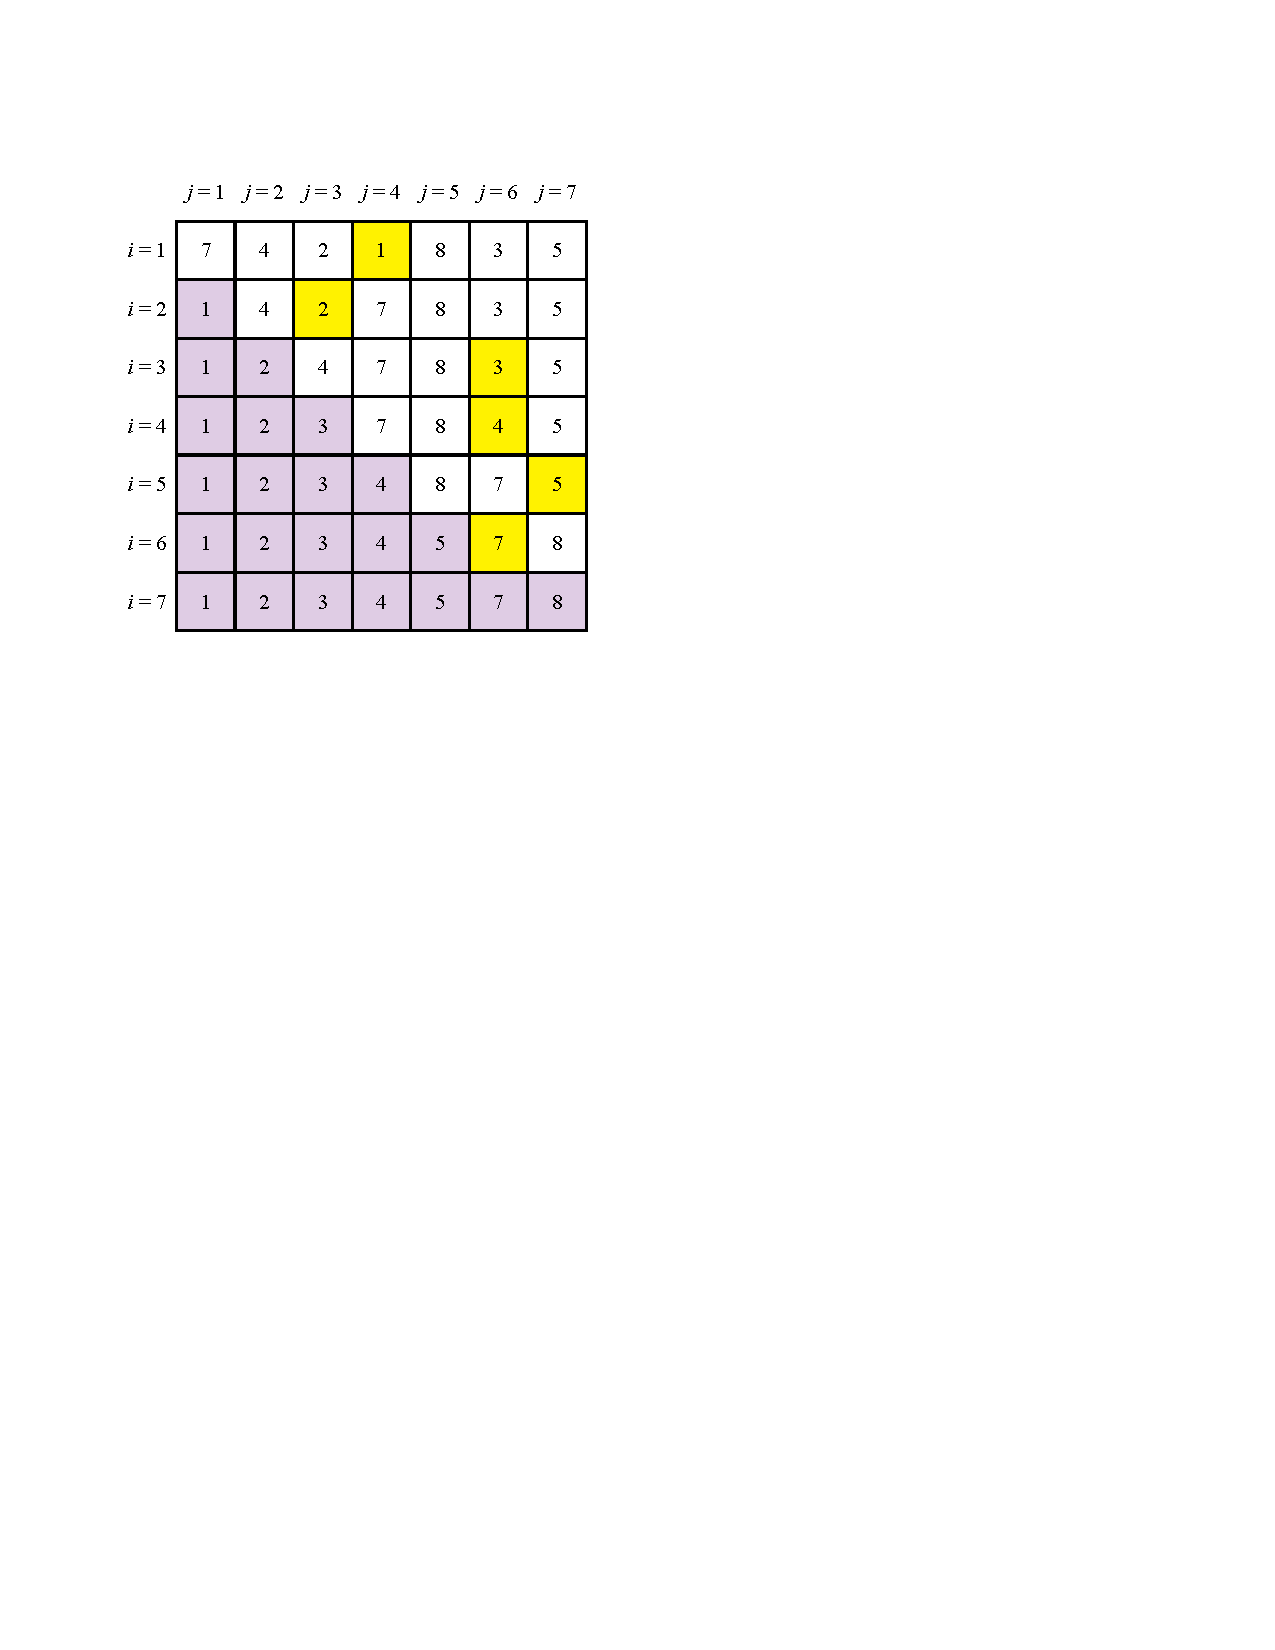
\includegraphics[width=\textwidth]{selection.pdf}
}
	
	
	
\end{frame}

%-------------------------------------------------------------------------
\begin{frame}{Selection Sort}

\vspace{-15pt}
\TwoColsCustom{0.48}{0.50}{
\begin{Procedure}
\caption[A]{\textsf{SelectionSort}($\Item[\,]\ A$, \INTEGER $n$)}
\For{$i = 1$ \TO $n-1$}{
  \INTEGER $\Min = \MIN(A, i, n)$\;
  $A[i] \leftrightarrow A[\Min]$\;
}
\end{Procedure}
}{
\begin{Procedure}
\caption[A]{\INTEGER \textsf{min}($\Item[\,]\ A$, \INTEGER $i$, \INTEGER $n$)}{
  \% Posizione del minimo parziale\;
  \INTEGER $\Min = i$\;
  \For{$j = i+1$ \TO $n$}
  {
    \If{$A[j] < A[\Min]$}{ 
      \% Nuovo minimo parziale\;
      $\Min = j$ 
    }
  }
  \Return $\Min$
}
\end{Procedure}
}

Complessità nel caso medio, pessimo, ottimo? \pause
\[
  \sum_{i=1}^{n-1} (n-i) = \sum_{i=1}^{n-1} i = \frac{n(n-1)}{2} = n^2 - n/2 = O(n^2)
\]	

\end{frame}



\subsection{Insertion Sort}

%-------------------------------------------------------------------------
\begin{frame}{Insertion Sort}

\BI
\item Algoritmo efficiente per ordinare piccoli insiemi di elementi
\item Si basa sul principio di ordinamento di una "mano" di carte da gioco (e.g. scala quaranta)
\EI	
	
\begin{Procedure}
\caption[A]{\insertionsort($\Item[\,]\ A,\ \INTEGER\ n$)}
  \For{$i = 2$ \TO\ $n$}{
    $\Item\ \Temp = A[i]$\;
    $\INTEGER\ j = i$\;
    \While{$j > 1$ \AND\ $A[j-1]>\Temp$}
    {
      $A[j] = A[j-1]$\;
      $j = j-1$\;
    }
    $A[j] = \Temp$\;
  }
\end{Procedure}

	
\end{frame}

%-------------------------------------------------------------------------
\begin{frame}{Insertion Sort}

\begin{overprint}
\includegraphics<1|handout:1>[width=0.95\textwidth]{insertion1.pdf}
\includegraphics<2|handout:2>[width=0.95\textwidth]{insertion2.pdf}
\includegraphics<3|handout:3>[width=0.95\textwidth]{insertion3.pdf}
\end{overprint}
\end{frame}


%-------------------------------------------------------------------------
\begin{frame}{Correttezza e complessità}

\vspace{-9pt}
\begin{myboxtitle}[In questo algoritmo]
\BI
\item Il costo di esecuzione non dipende solo dalla dimensione...
\item ma anche dalla distribuzione dei dati in ingresso
\EI
\end{myboxtitle}

\begin{myboxtitle}[Domande]
\BI
\item Dimostrare che l'algoritmo è corretto
\item Qual è il costo nel caso il vettore sia già ordinato?
\item Qual è il costo nel caso il vettore sia ordinato in ordine inverso?
\item Cosa succede "in media"? (informalmente)
\EI
\end{myboxtitle}

\end{frame}

\subsection{Merge Sort}

%-------------------------------------------------------------------------
\begin{frame}{Merge Sort}
	
\vspace{-9pt}
\begin{myboxtitle}[Divide et impera]
Merge Sort è basato sulla tecnica \alert{divide-et-impera} vista in precedenza	
\BI
\item \alert{Divide}: Spezza virtualmente il vettore di $n$ elementi in due sottovettori di $n/2$ elementi
\item \alert{Impera}: Chiama Merge Sort ricorsivamente sui due sottovettori
\item \alert{Combina}: Unisci (\alert{merge}) le due sequenze ordinate 
\EI
\end{myboxtitle}

\begin{myboxtitle}[Idea]
Si sfrutta il fatto che i due sottovettori sono già ordinati per ordinare più velocemente
\end{myboxtitle}
	
\end{frame}



%-------------------------------------------------------------------------
\begin{frame}[shrink]{Merge}

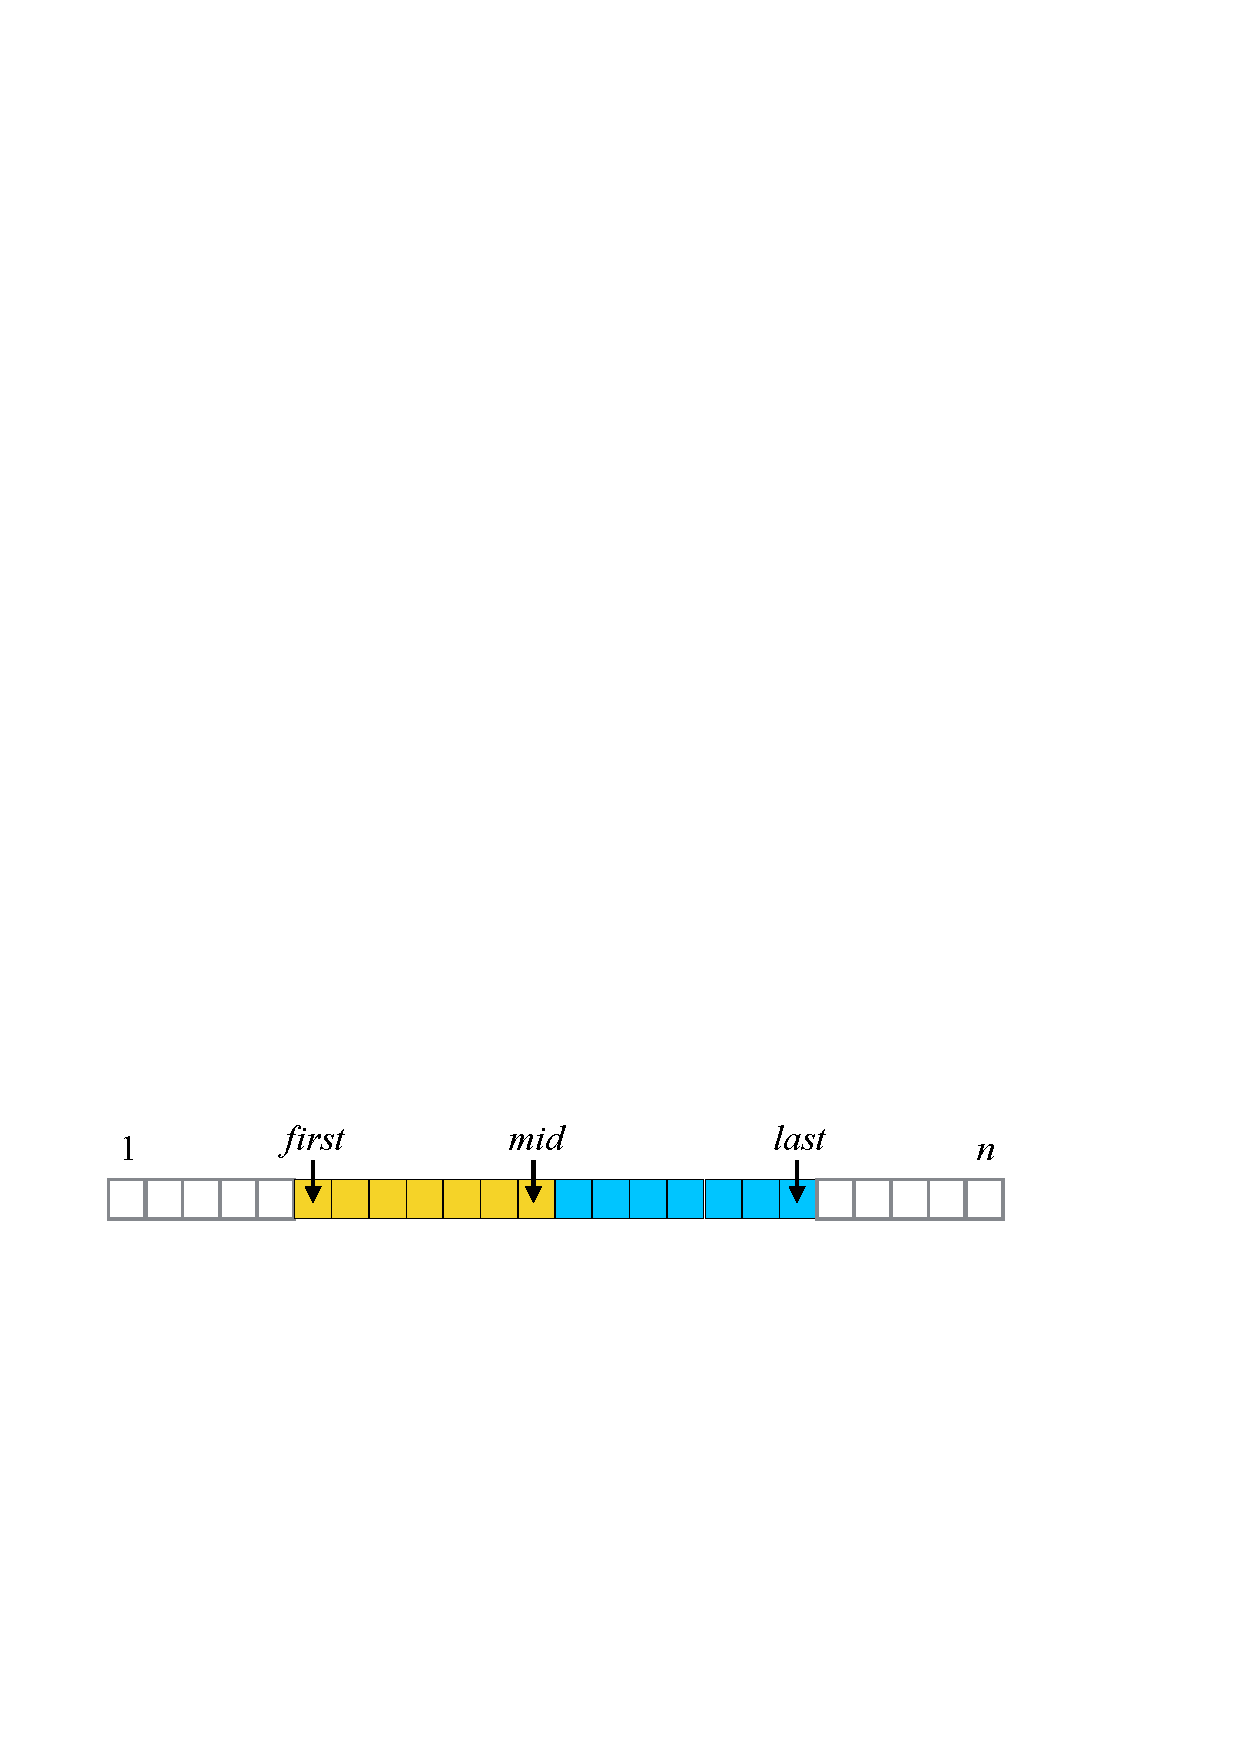
\includegraphics[width=\textwidth]{merge.pdf}
\bigskip	
% \begin{myboxtitle}[$\Merge(\INTEGER[\,]\ A, \INTEGER\ \Primo, \INTEGER\ \Ultimo, \INTEGER\ \Mezzo)$]
\textbf{Input}:
\BI
\item $A$ è un vettore di $n$ interi
\item $\Primo, \Ultimo$, $\Mezzo$ sono tali che 
$1 \leq \Primo \leq \Mezzo < \Ultimo \leq n$
\item I sottovettori $A[\Primo \ldots \Mezzo]$ e $A[\Mezzo+1 \ldots \Ultimo]$ sono già ordinati
\EI
\textbf{Output}:
\BI
\item I due sottovettori sono fusi in un unico sottovettore ordinato A[\Primo \ldots \Ultimo] tramite un vettore di appoggio $B$
\EI
% \end{myboxtitle}


\end{frame}

%-------------------------------------------------------------------------
\begin{frame}{Funzionamento \textsf{Merge}()}

\begin{center}
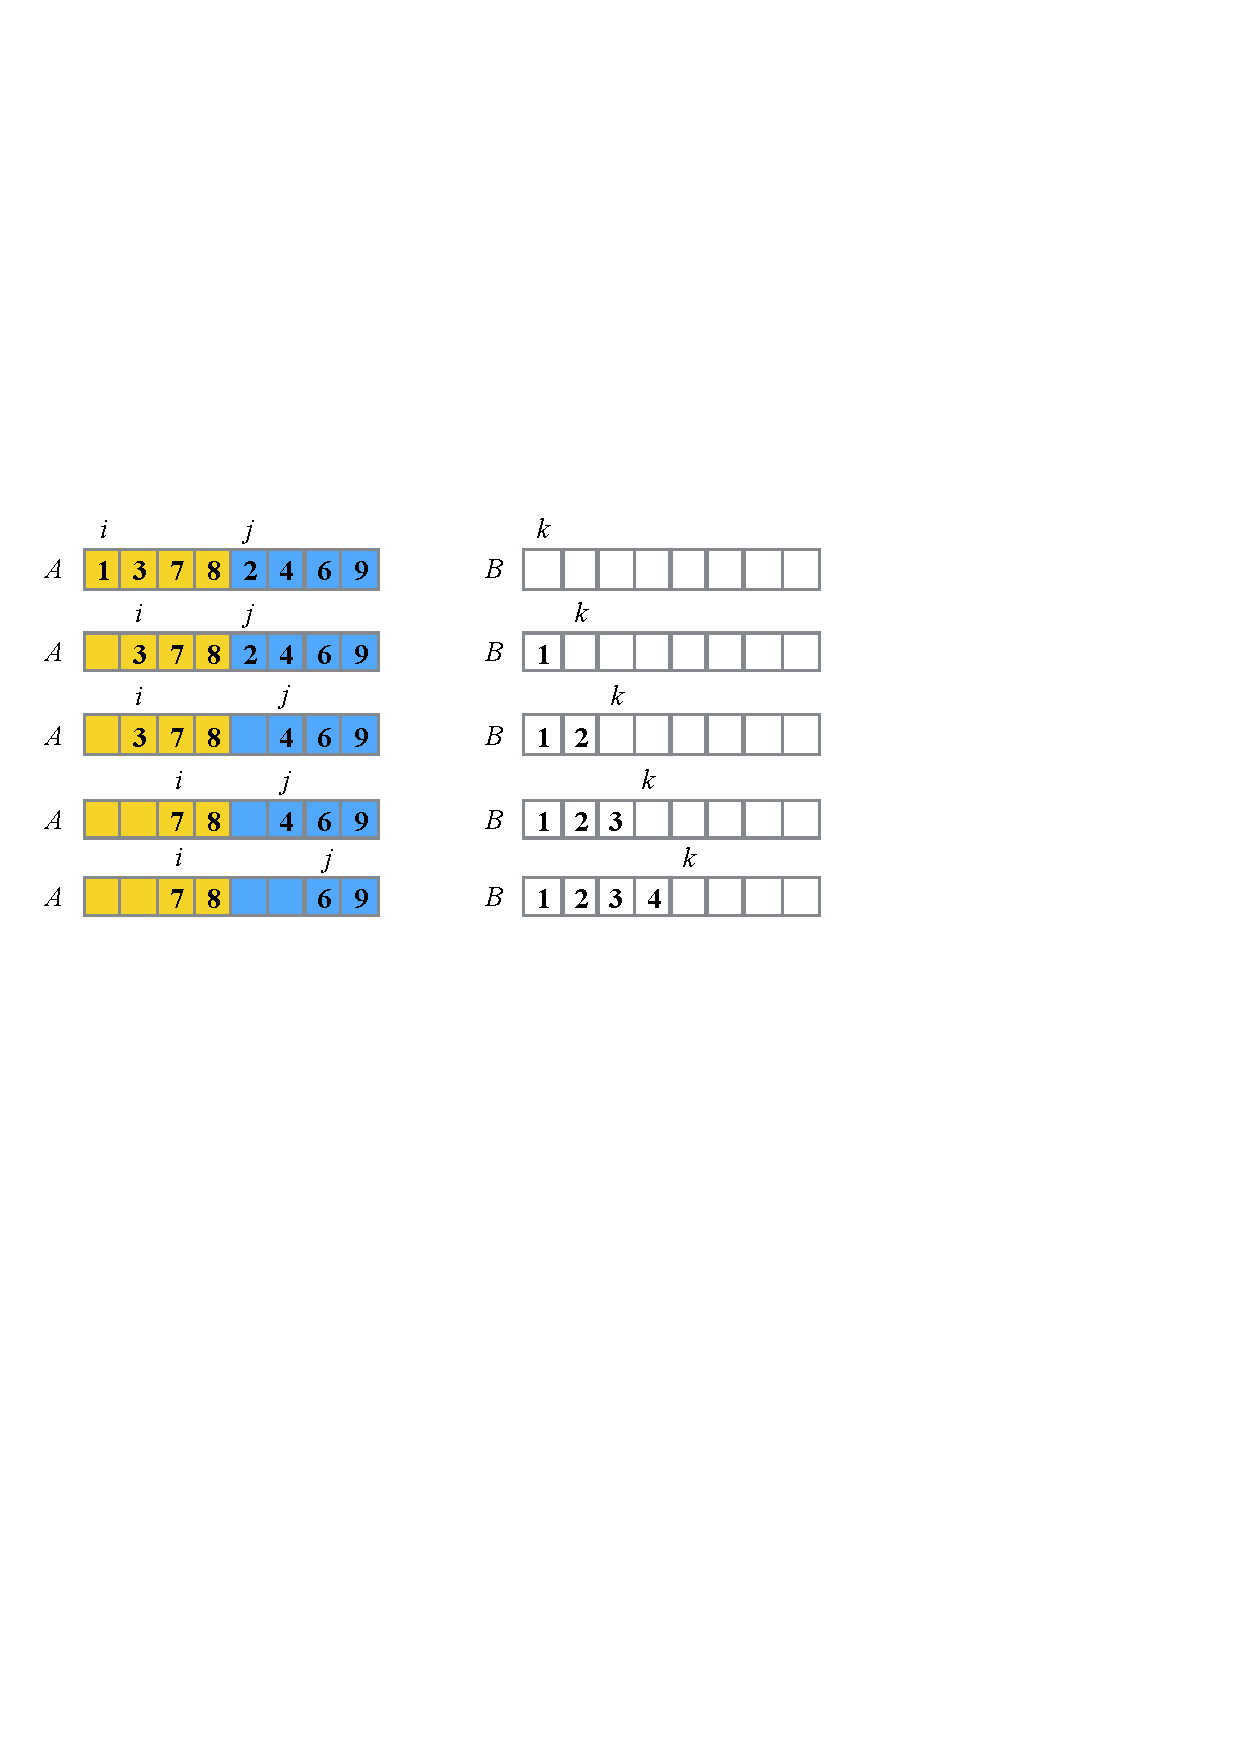
\includegraphics[width=\textwidth]{merge2.pdf}
\end{center}

\end{frame}

%-------------------------------------------------------------------------
\begin{frame}{Funzionamento \textsf{Merge}()}

\begin{center}
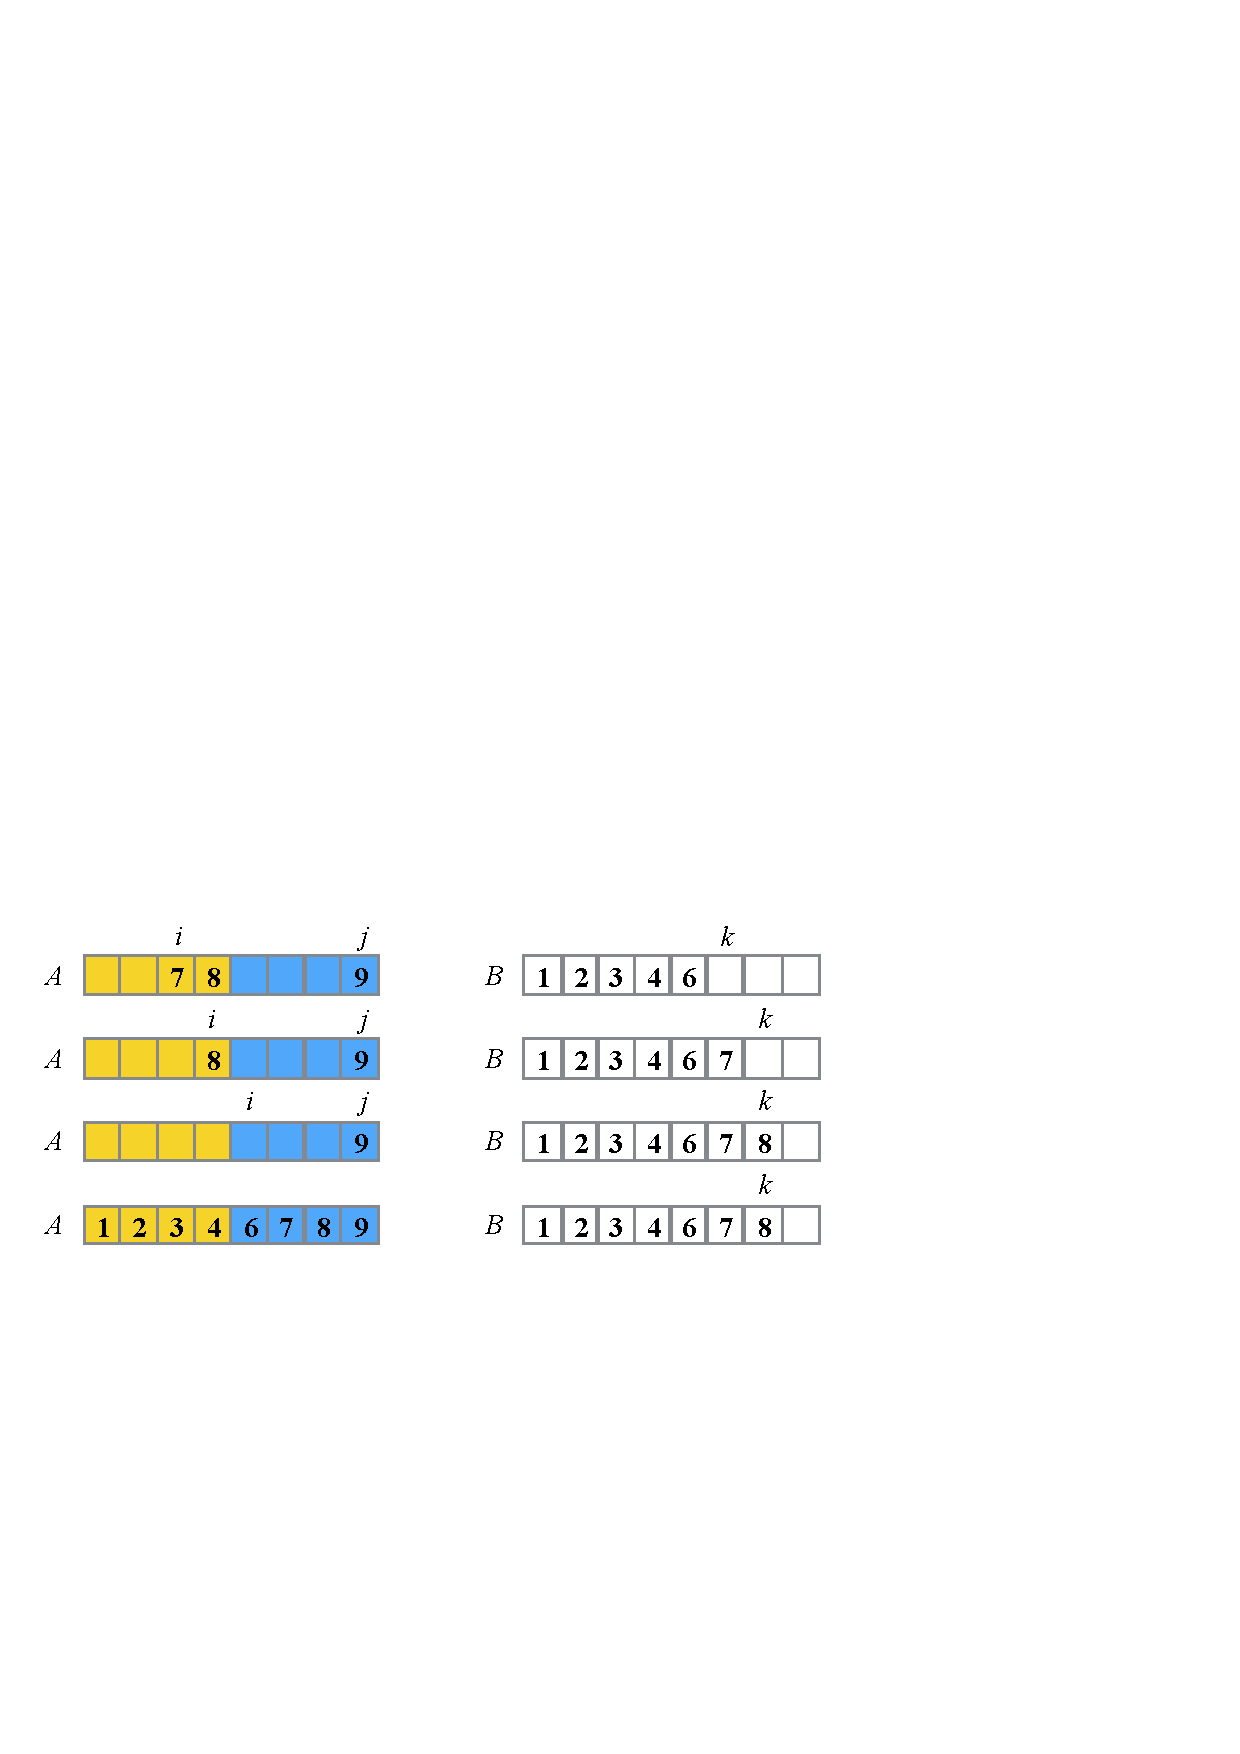
\includegraphics[width=\textwidth]{merge3.pdf}
\end{center}

\end{frame}

%-------------------------------------------------------------------------
\begin{frame}[shrink=6]{\textsf{Merge}()}
	
\vspace{-12pt}
\begin{Procedure}
\caption[A]{\Merge($\Item\ A[\,]$, \INTEGER\ \Primo, \INTEGER\ \Ultimo, \INTEGER \Mezzo)}
\begin{multicols}{2}
  \INTEGER $i$, $j$, $k$, $h$\;
  $i = \Primo$\;
	$j = \Mezzo+1$\;
	$k = \Primo$\;
  \While{$i \leq \Mezzo\ \AND\ j \leq \Ultimo$}
  {
    \eIf{$A[i] \leq A[j]$}
    {
      $B[k] = A[i]$\;
      $i = i+1$\;
    }
    {
      $B[k] = A[j]$\;
      $j = j+1$\;
    }
    $k = k+1$\;
  }
  $j = \Ultimo$\;
  \For{$h = \Mezzo$ \DOWNTO $i$}
  {
    $A[j] = A[h]$\;
    $j = j-1$\;
  }
  \For{$j = \Primo$ \TO\ $k-1$}
  {
    $A[j] = B[j]$\;
  }
\end{multicols}
\BlankLine
\BlankLine
\end{Procedure}

\end{frame}

%-------------------------------------------------------------------------
\begin{frame}{Costo computazionale}

\vspace{-9pt}
\begin{myboxtitle}[Domanda]
	Qual è il costo computazionale di \Merge()? \pause $\Rightarrow \alert{O(n)}$
\end{myboxtitle}

\end{frame}

%-------------------------------------------------------------------------
\begin{frame}{MergeSort}
Programma completo:
\BI
\item Chiama ricorsivamente se stesso e usa \Merge() per unire i risultati
\item Caso base: sequenze di lunghezza $\leq 1$ sono già ordinate
\EI	
\bigskip
\begin{Procedure}
\caption[A]{\Mergesort($\Item\ A[\ ]$, \INTEGER \Primo, \INTEGER \Ultimo)}

  \If{$\Primo < \Ultimo$}
  {
    \INTEGER $\Mezzo = \lfloor(\Primo + \Ultimo) / 2\rfloor$ \;
	$\Mergesort(A, \Primo, \Mezzo)$ \;
	$\Mergesort(A, \Mezzo + 1, \Ultimo)$ \;
	$\Merge(A, \Primo, \Ultimo, \Mezzo)$ \;
  }	
\end{Procedure}

\end{frame}

%-------------------------------------------------------------------------
\begin{frame}{\textsf{MergeSort}(): Esecuzione}
\begin{overprint}
\includegraphics<1|handout:1>[width=\textwidth,page=1]{merge-crop.pdf}
\includegraphics<2|handout:0>[width=\textwidth,page=2]{merge-crop.pdf}
\includegraphics<3|handout:0>[width=\textwidth,page=3]{merge-crop.pdf}
\includegraphics<4|handout:0>[width=\textwidth,page=4]{merge-crop.pdf}
\includegraphics<5|handout:0>[width=\textwidth,page=5]{merge-crop.pdf}
\includegraphics<6|handout:0>[width=\textwidth,page=6]{merge-crop.pdf}
\includegraphics<7|handout:0>[width=\textwidth,page=7]{merge-crop.pdf}
\includegraphics<8|handout:0>[width=\textwidth,page=8]{merge-crop.pdf}
\includegraphics<9|handout:0>[width=\textwidth,page=9]{merge-crop.pdf}
\includegraphics<10|handout:0>[width=\textwidth,page=10]{merge-crop.pdf}
\includegraphics<11|handout:0>[width=\textwidth,page=11]{merge-crop.pdf}
\includegraphics<12|handout:0>[width=\textwidth,page=12]{merge-crop.pdf}
\includegraphics<13|handout:0>[width=\textwidth,page=13]{merge-crop.pdf}
\includegraphics<14|handout:0>[width=\textwidth,page=14]{merge-crop.pdf}
\includegraphics<15|handout:0>[width=\textwidth,page=15]{merge-crop.pdf}
\includegraphics<16|handout:0>[width=\textwidth,page=16]{merge-crop.pdf}
\includegraphics<17|handout:0>[width=\textwidth,page=17]{merge-crop.pdf}
\includegraphics<18|handout:0>[width=\textwidth,page=18]{merge-crop.pdf}
\includegraphics<19|handout:0>[width=\textwidth,page=19]{merge-crop.pdf}
\includegraphics<20|handout:0>[width=\textwidth,page=20]{merge-crop.pdf}
\includegraphics<21|handout:0>[width=\textwidth,page=21]{merge-crop.pdf}
\includegraphics<22|handout:0>[width=\textwidth,page=22]{merge-crop.pdf}
\includegraphics<23|handout:0>[width=\textwidth,page=23]{merge-crop.pdf}
\includegraphics<24|handout:0>[width=\textwidth,page=24]{merge-crop.pdf}
\includegraphics<25|handout:0>[width=\textwidth,page=25]{merge-crop.pdf}
\includegraphics<26|handout:0>[width=\textwidth,page=26]{merge-crop.pdf}
\includegraphics<27|handout:0>[width=\textwidth,page=27]{merge-crop.pdf}
\includegraphics<28|handout:0>[width=\textwidth,page=28]{merge-crop.pdf}
\includegraphics<29|handout:0>[width=\textwidth,page=29]{merge-crop.pdf}
\includegraphics<30|handout:0>[width=\textwidth,page=30]{merge-crop.pdf}
\includegraphics<31|handout:0>[width=\textwidth,page=31]{merge-crop.pdf}
\includegraphics<32|handout:0>[width=\textwidth,page=32]{merge-crop.pdf}
\includegraphics<33|handout:0>[width=\textwidth,page=33]{merge-crop.pdf}
\includegraphics<34|handout:0>[width=\textwidth,page=34]{merge-crop.pdf}
\includegraphics<35|handout:0>[width=\textwidth,page=35]{merge-crop.pdf}
\includegraphics<36|handout:0>[width=\textwidth,page=36]{merge-crop.pdf}
\includegraphics<37|handout:0>[width=\textwidth,page=37]{merge-crop.pdf}
\includegraphics<38|handout:0>[width=\textwidth,page=38]{merge-crop.pdf}
\includegraphics<39|handout:0>[width=\textwidth,page=39]{merge-crop.pdf}
\includegraphics<40|handout:0>[width=\textwidth,page=40]{merge-crop.pdf}
\includegraphics<41|handout:0>[width=\textwidth,page=41]{merge-crop.pdf}
\includegraphics<42|handout:0>[width=\textwidth,page=42]{merge-crop.pdf}
\includegraphics<43|handout:0>[width=\textwidth,page=43]{merge-crop.pdf}
\includegraphics<44|handout:0>[width=\textwidth,page=44]{merge-crop.pdf}
\includegraphics<45|handout:0>[width=\textwidth,page=45]{merge-crop.pdf}
\includegraphics<46|handout:0>[width=\textwidth,page=46]{merge-crop.pdf}
\includegraphics<47|handout:0>[width=\textwidth,page=47]{merge-crop.pdf}
\includegraphics<48|handout:0>[width=\textwidth,page=48]{merge-crop.pdf}
\includegraphics<49|handout:0>[width=\textwidth,page=49]{merge-crop.pdf}
\includegraphics<50|handout:0>[width=\textwidth,page=50]{merge-crop.pdf}
\includegraphics<51|handout:0>[width=\textwidth,page=51]{merge-crop.pdf}
\includegraphics<52|handout:0>[width=\textwidth,page=52]{merge-crop.pdf}
\includegraphics<53|handout:0>[width=\textwidth,page=53]{merge-crop.pdf}
\includegraphics<54|handout:0>[width=\textwidth,page=54]{merge-crop.pdf}
\includegraphics<55|handout:2>[width=\textwidth,page=55]{merge-crop.pdf}
\end{overprint}
\end{frame}


%-------------------------------------------------------------------------
\begin{frame}{Analisi di \textsf{MergeSort}()}
Un'assunzione semplificativa:
\BI
\item $n = 2^k$, ovvero l'altezza dell'albero di suddivisioni è esattamente $k = \log n$;
\item Tutti i sottovettori hanno dimensioni che sono potenze esatte di $2$
\EI

\bigskip
\begin{myboxtitle}[Costo computazionale]
\[
  T(n) = \begin{cases}
    c & n=1 \\
	2T(n/2) + dn  & n>1
  \end{cases}
\]
\end{myboxtitle}


\end{frame}

%-------------------------------------------------------------------------
\begin{frame}{Costo computazionale di Merge Sort}

\vspace{-12pt}
\begin{myboxtitle}[Domanda]
	Qual è il costo computazionale di \Mergesort()?  
\end{myboxtitle}

\pause
\begin{overprint}
\includegraphics<2|handout:0>[width=\textwidth]{merge-sort-recursion-tree1.pdf}
\includegraphics<3|handout:2>[width=\textwidth]{merge-sort-recursion-tree2.pdf}
\end{overprint}

\end{frame}

%-------------------------------------------------------------------------
\begin{frame}{Un po' di storia}

\TwoColsCustom{0.65}{0.32}{
\BI
\item Il censimento americano del 1880 aveva richiesto otto anni per essere
completato
\item Quello del 1890 richiese sei settimane, grazie alla Hollerith Machine
\item Fra il 1896 e il 1924, la Hollerith \& Co ha cambiato diversi nomi. L'ultimo? \\
\alert{International Business Machines}
\item Le Collating Machines (1936) prendevano
due stack di schede perforate ordinate e le ordinavano in un unico stack
\item Nel 1945-48, John von Neumann descrisse per la prima volta il MergeSort partendo dall'idea delle Collating Machines.
\end{itemize}
}{
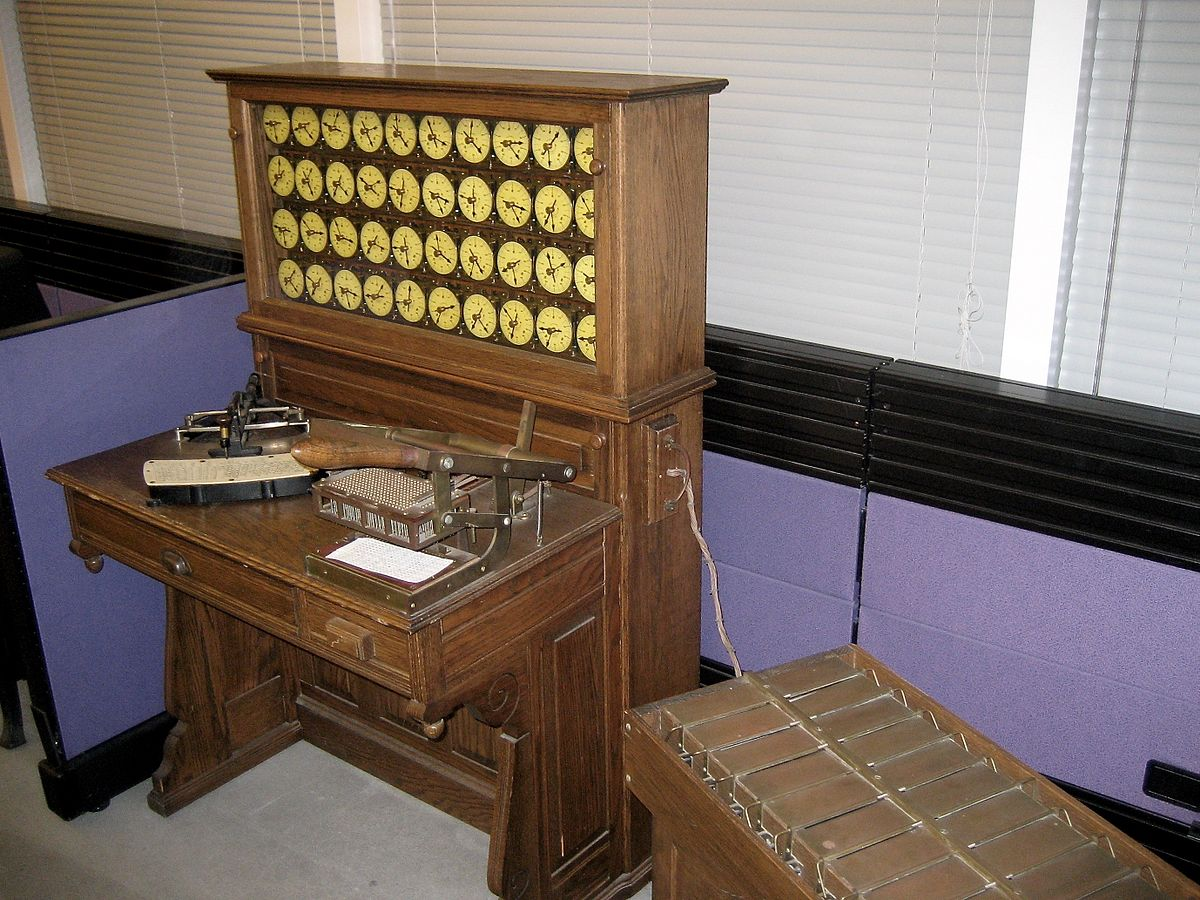
\includegraphics[width=\textwidth]{hollerith.jpg}

\smallskip
Hollerith Machine
}

\end{frame}


%-------------------------------------------------------------------------
\begin{OnlySlides}{MergeSort, in pillole}
\begin{center}
    \IG{1.0}{merge-sort.png}
\end{center}
\end{OnlySlides}


%-------------------------------------------------------------------------
\begin{OnlySlides}{Ricorsione}

\setlength\epigraphwidth{.60\textwidth}
\epigraph{\alert{Recursion is the root of computation because it trades description for time.}
}{\textit{Alan Perlis, Epigrams on Programming}}


\begin{center}
\IG{0.8}{google-recursion.jpg}
\end{center}

\end{OnlySlides}

\end{document}


